% ------------------------------------------------------------

% LaTeX Template für die DHBW zum Schnellstart!
% Original: https://github.wdf.sap.corp/vtgermany/LaTeX-Template-DHBW
% ------------------------------------------------------------
% ---- Präambel mit Angaben zum Dokument
\documentclass[
	fontsize=12pt,           % Leitlinien sprechen von Schriftgröße 12.
	paper=A4,
	twoside=false,
	listof=totoc,            % Tabellen- und Abbildungsverzeichnis ins Inhaltsverzeichnis
	bibliography=totoc,      % Literaturverzeichnis ins Inhaltsverzeichnis aufnehmen
	titlepage,               % Titlepage-Umgebung anstatt \maketitle
	headsepline,             % horizontale Linie unter Kolumnentitel
	abstract,              % Überschrift einschalten, Abstract muss in {abstract}-Umgebung stehen
]{scrreprt}                  % Verwendung von KOMA-Report
\usepackage[utf8]{inputenc}  % UTF8 Encoding einschalten
\usepackage[ngerman]{babel}  % Neue deutsche Rechtschreibung
\usepackage[T1]{fontenc}     % Ausgabe von westeuropäischen Zeichen (auch Umlaute)
\usepackage{microtype}       % Trennung von Wörtern wird besser umgesetzt
\usepackage{lmodern}         % Nicht-gerasterte Schriftarten (bei MikTeX erforderlich)
\usepackage{graphicx}        % Einbinden von Grafiken erlauben
\usepackage{wrapfig}         % Grafiken fließend im Text
\usepackage{setspace}        % Zeilenabstand \singlespacing, \onehalfspaceing, \doublespacing
\usepackage[
	%showframe,                % Ränder anzeigen lassen
	left=2.7cm, right=2.5cm,
	top=2.5cm,  bottom=2.5cm,
	includeheadfoot
]{geometry}                      % Seitenlayout einstellen
\usepackage{scrlayer-scrpage}    % Gestaltung von Fuß- und Kopfzeilen
\usepackage{acronym}             % Abkürzungen, Abkürzungsverzeichnis
\usepackage{titletoc}            % Anpassungen am Inhaltsverzeichnis
\contentsmargin{0.75cm}          % Abstand im Inhaltsverzeichnis zw. Punkt und Seitenzahl
\usepackage[                     % Klickbare Links (enth. auch "nameref", "url" Package)
  hidelinks,                     % Blende die "URL Boxen" aus.
  breaklinks=true                % Breche zu lange URLs am Zeilenende um
]{hyperref}
\usepackage[hypcap=true]{caption}% Anker Anpassung für Referenzen

\usepackage{lineno}

\usepackage{chngcntr}
\counterwithout{figure}{chapter}

\renewcommand{\thefigure}{\arabic{figure}}
\renewcommand{\thetable}{\arabic{table}}

\urlstyle{same}                  % Aktuelle Schrift auch für URLs
% Anpassung von autoref für Gleichungen (ergänzt runde Klammern) und Algorithm.
% Anstatt "Listing" kann auch z.B. "Code-Ausschnitt" verwendet werden. Dies sollte
% jedoch synchron gehalten werden mit \lstlistingname (siehe weiter unten).
\addto\extrasngerman{%
	\def\equationautorefname~#1\null{Gleichung~(#1)\null}
	\def\lstnumberautorefname{Zeile}
	\def\lstlistingautorefname{Listing}
	\def\algorithmautorefname{Algorithmus}
	% Damit einheitlich "Abschnitt 1.2[.3]" verwendet wird und nicht "Unterabschnitt 1.2.3"
	% \def\subsectionautorefname{Abschnitt}
}

% ---- Abstand verkleinern von der Überschrift 
\renewcommand*{\chapterheadstartvskip}{\vspace*{.5\baselineskip}}

% Hierdurch werden Schusterjungen und Hurenkinder vermieden, d.h. einzelne Wörter
% auf der nächsten Seite oder in einer einzigen Zeile.
% LaTeX kann diese dennoch erzeugen, falls das Layout ansonsten nicht umsetzbar ist.
% Diese Werte sind aber gute Startwerte.
\widowpenalty10000
\clubpenalty10000

% ---- Für das Quellenverzeichnis
\usepackage[
	backend = biber,                % Verweis auf biber
	language = auto,
	style = numeric,                % Nummerierung der Quellen mit Zahlen
	citestyle=authoryear,
	sorting = none,                 % none = Sortierung nach der Erscheinung im Dokument
	sortcites = true,               % Sortiert die Quellen innerhalb eines cite-Befehls
	block = space,                  % Extra Leerzeichen zwischen Blocks
	hyperref = true,                % Links sind klickbar auch in der Quelle
	%backref = true,                % Referenz, auf den Text an die zitierte Stelle
	bibencoding = auto,
	giveninits = true,              % Vornamen werden abgekürzt
	doi=false,                      % DOI nicht anzeigen
	isbn=false,                     % ISBN nicht anzeigen
    alldates=short                  % Datum immer als DD.MM.YYYY anzeigen
]{biblatex}
\addbibresource{Inhalt/literatur.bib}
\setcounter{biburlnumpenalty}{3000}     % Umbruchgrenze für Zahlen
\setcounter{biburlucpenalty}{6000}      % Umbruchgrenze für Großbuchstaben
\setcounter{biburllcpenalty}{9000}      % Umbruchgrenze für Kleinbuchstaben
\DeclareNameAlias{default}{family-given}  % Nachname vor dem Vornamen
\AtBeginBibliography{\renewcommand{\multinamedelim}{\addslash\space
}\renewcommand{\finalnamedelim}{\multinamedelim}}  % Schrägstrich zwischen den Autorennamen
\DefineBibliographyStrings{german}{
  urlseen = {Einsichtnahme:},                      % Ändern des Titels von "besucht am"
}
\usepackage[babel,german=quotes]{csquotes}         % Deutsche Anführungszeichen + Zitate


\usepackage{xcolor}
\usepackage{blindtext}
\usepackage{soul}

% ---- Für Mathevorlage
\usepackage{amsmath}    % Erweiterung vom Mathe-Satz
\usepackage{amssymb}    % Lädt amsfonts und weitere Symbole
\usepackage{MnSymbol}   % Für Symbole, die in amssymb nicht enthalten sind.


% ---- Für Quellcodevorlage
\usepackage{scrhack}                    % Hack zur Verw. von listings in KOMA-Script
\usepackage{listings}                   % Darstellung von Quellcode
\usepackage{xcolor}                     % Einfache Verwendung von Farben
% -- Eigene Farben für den Quellcode
\definecolor{JavaLila}{rgb}{0.4,0.1,0.4}
\definecolor{JavaGruen}{rgb}{0.3,0.5,0.4}
\definecolor{JavaBlau}{rgb}{0.0,0.0,1.0}
\definecolor{ABAPKeywordsBlue}{HTML}{6000ff}
\definecolor{ABAPCommentGrey}{HTML}{808080}
\definecolor{ABAPStringGreen}{HTML}{4da619}
\definecolor{PyKeywordsBlue}{HTML}{0000AC}
\definecolor{PyCommentGrey}{HTML}{808080}
\definecolor{PyStringGreen}{HTML}{008080}
% -- Farben für ABAP CDS
\definecolor{CDSString}{HTML}{FF8C00}
\definecolor{CDSKeywords}{HTML}{6000ff}
\definecolor{CDSAnnotation}{HTML}{00BFFF}
\definecolor{CDSComment}{HTML}{808080}
\definecolor{CDSFunc}{HTML}{FF0000}

% -- Default Listing-Styles

\lstset{
	% Das Paket "listings" kann kein UTF-8. Deswegen werden hier 
	% die häufigsten Zeichen definiert (ä,ö,ü,...)
	literate=%
		{á}{{\'a}}1 {é}{{\'e}}1 {í}{{\'i}}1 {ó}{{\'o}}1 {ú}{{\'u}}1
		{Á}{{\'A}}1 {É}{{\'E}}1 {Í}{{\'I}}1 {Ó}{{\'O}}1 {Ú}{{\'U}}1
		{à}{{\`a}}1 {è}{{\`e}}1 {ì}{{\`i}}1 {ò}{{\`o}}1 {ù}{{\`u}}1
		{À}{{\`A}}1 {È}{{\'E}}1 {Ì}{{\`I}}1 {Ò}{{\`O}}1 {Ù}{{\`U}}1
		{ä}{{\"a}}1 {ë}{{\"e}}1 {ï}{{\"i}}1 {ö}{{\"o}}1 {ü}{{\"u}}1
		{Ä}{{\"A}}1 {Ë}{{\"E}}1 {Ï}{{\"I}}1 {Ö}{{\"O}}1 {Ü}{{\"U}}1
		{â}{{\^a}}1 {ê}{{\^e}}1 {î}{{\^i}}1 {ô}{{\^o}}1 {û}{{\^u}}1
		{Â}{{\^A}}1 {Ê}{{\^E}}1 {Î}{{\^I}}1 {Ô}{{\^O}}1 {Û}{{\^U}}1
		{œ}{{\oe}}1 {Œ}{{\OE}}1 {æ}{{\ae}}1 {Æ}{{\AE}}1 {ß}{{\ss}}1
		{ű}{{\H{u}}}1 {Ű}{{\H{U}}}1 {ő}{{\H{o}}}1 {Ő}{{\H{O}}}1
		{ç}{{\c c}}1 {Ç}{{\c C}}1 {ø}{{\o}}1 {å}{{\r a}}1 {Å}{{\r A}}1
		{€}{{\euro}}1 {£}{{\pounds}}1 {«}{{\guillemotleft}}1
		{»}{{\guillemotright}}1 {ñ}{{\~n}}1 {Ñ}{{\~N}}1 {¿}{{?`}}1,
	breaklines=true,        % Breche lange Zeilen um 
	breakatwhitespace=true, % Wenn möglich, bei Leerzeichen umbrechen
	% Symbol für Zeilenumbruch einfügen
	prebreak=\raisebox{0ex}[0ex][0ex]{\ensuremath{\rhookswarrow}},
	postbreak=\raisebox{0ex}[0ex][0ex]{\ensuremath{\rcurvearrowse\space}},
	tabsize=4,                                 % Setze die Breite eines Tabs
	basicstyle=\ttfamily\small,                % Grundsätzlicher Schriftstyle
	columns=fixed,                             % Besseres Schriftbild
	numbers=left,                              % Nummerierung der Zeilen
	%frame=single,                             % Umrandung des Codes
	showstringspaces=false,                    % Keine Leerzeichen hervorheben
	keywordstyle=\color{blue},
	ndkeywordstyle=\bfseries\color{darkgray},
	identifierstyle=\color{black},
	commentstyle=\itshape\color{JavaGruen},   % Kommentare in eigener Farbe
	stringstyle=\color{JavaBlau},             % Strings in eigener Farbe,
	captionpos=b,                             % Bild*unter*schrift
	xleftmargin=5.0ex
}

% ---- Eigener JAVA-Style für den Quellcode
\renewcommand{\ttdefault}{pcr}               % Schriftart, welche auch fett beinhaltet
\lstdefinestyle{EigenerJavaStyle}{
	language=Java,                             % Syntax Highlighting für Java
	%frame=single,                             % Umrandung des Codes
	keywordstyle=\bfseries\color{JavaLila},    % Keywords in eigener Farbe und fett
	commentstyle=\itshape\color{JavaGruen},    % Kommentare in eigener Farbe und italic
	stringstyle=\color{JavaBlau}               % Strings in eigener Farbe
}

% ---- Eigener ABAP-Style für den Quellcode
\renewcommand{\ttdefault}{pcr}
\lstdefinestyle{EigenerABAPStyle}{
	language=[R/3 6.10]ABAP,
	morestring=[b]\|,                          % Für Pipe-Strings
	morestring=[b]\`,                          % für Backtick-Strings
	keywordstyle=\bfseries\color{ABAPKeywordsBlue},
	commentstyle=\itshape\color{ABAPCommentGrey},
	stringstyle=\color{ABAPStringGreen},
	tabsize=2,
	morekeywords={
		types,
		@data,
		as,
		lower,
		start,
		selection,
		order,
		by,
		inner,
		join,
		key,
		end,
		cast
	}
}

% ---- Eigener Python-Style für den Quellcode
\renewcommand{\ttdefault}{pcr}
\lstdefinestyle{EigenerPythonStyle}{
	language=Python,
	columns=flexible,
	keywordstyle=\bfseries\color{PyKeywordsBlue},
	commentstyle=\itshape\color{PyCommentGrey},
	stringstyle=\color{PyStringGreen}
}

%----- ABAP-CDS-View language
\lstdefinelanguage{ABAPCDS}{
	sensitive=false,
	%Keywords
	morekeywords={define,
		view,
		as,
		select,
		from,
		inner,
		join,
		on,
		key,
		case,
		when,
		then,
		else,
		end,
		true,
		false,
		cast,
		where,
		and,
		distinct,
		group,
		by,
		having,
		min,
		sum,
		max,
		count,
		avg
	},
	%Methoden
	morekeywords=[2]{
		div,
		currency\_conversion,
		dats\_days\_between,
		concat\_with\_space,
		dats\_add_days,
		dats\_is\_valid,
		dats\_add\_months,
		unit\_conversion,
		division,
		mod,
		abs,
		floor,
		ceil,
		round,
		concat,
		replace,
		substring,
		left,
		right,
		length
	},
	morecomment=[s][\color{CDSAnnotation}]{@}{:},
	morecomment=[l][\itshape\color{CDSComment}]{//},
	morecomment=[s][\itshape\color{CDSComment}]{/*}{*/},
	morestring=[b][\color{CDSString}]',
	keywordstyle=\bfseries\color{CDSKeywords},
	keywordstyle=[2]\color{CDSFunc}
}

  % Weitere Details sind ausgelagert

\usepackage{algorithm}                  % Für Algorithmen-Umgebung (ähnlich wie lstlistings Umgebung)
\usepackage{algpseudocode}              % Für Pseudocode. Füge "[noend]" hinzu, wenn du kein "endif",
                                        % etc. haben willst.

\makeatletter                           % Sorgt dafür, dass man @ in Namen verwenden kann.
                                        % Ansonsten gibt es in der nächsten Zeile einen Compilefehler.
\renewcommand{\ALG@name}{Algorithmus}   % Umbenennen von "Algorithm" im Header der Listings.
\makeatother                            % Zeichen wieder zurücksetzen
\renewcommand{\lstlistingname}{Listing} % Erlaubt das Umbenennen von "Listing" in anderen Titel.

% ---- Tabellen
\usepackage{booktabs}  % Für schönere Tabellen. Enthält neue Befehle wie \midrule
\usepackage{multirow}  % Mehrzeilige Tabellen
\usepackage{siunitx}   % Für SI Einheiten und das Ausrichten Nachkommastellen
\sisetup{locale=DE, range-phrase={~bis~}, output-decimal-marker={,}} % Damit ein Komma und kein Punkt verwendet wird.
\usepackage{xfrac} % Für siunitx Option "fraction-function=\sfrac"

% ---- Für Definitionsboxen in der Einleitung
\usepackage{amsthm}                     % Liefert die Grundlagen für Theoreme
\usepackage[framemethod=tikz]{mdframed} % Boxen für die Umrandung
% ---- Definition für Highlight Boxen

% ---- Grundsätzliche Definition zum Style
\newtheoremstyle{defi}
  {\topsep}         % Abstand oben
  {\topsep}         % Abstand unten
  {\normalfont}     % Schrift des Bodys
  {0pt}             % Einschub der ersten Zeile
  {\bfseries}       % Darstellung von der Schrift in der Überschrift
  {:}               % Trennzeichen zwischen Überschrift und Body
  {.5em}            % Abstand nach dem Trennzeichen zum Body Text
  {\thmname{#3}}    % Name in eckigen Klammern
\theoremstyle{defi}

% ------ Definition zum Strich vor eines Texts
\newmdtheoremenv[
  hidealllines = true,       % Rahmen komplett ausblenden
  leftline = true,           % Linie links einschalten
  innertopmargin = 0pt,      % Abstand oben
  innerbottommargin = 4pt,   % Abstand unten
  innerrightmargin = 0pt,    % Abstand rechts
  linewidth = 3pt,           % Linienbreite
  linecolor = gray!40,       % Linienfarbe
]{defStrich}{Definition}     % Name der des formats "defStrich"

% ------ Definition zum Eck-Kasten um einen Text
\newmdtheoremenv[
  hidealllines = true,
  innertopmargin = 6pt,
  linecolor = gray!40,
  singleextra={              % Eck-Markierungen für die Definition
    \draw[line width=3pt,gray!50,line cap=rect] (O|-P) -- +(1cm,0pt);
    \draw[line width=3pt,gray!50,line cap=rect] (O|-P) -- +(0pt,-1cm);
    \draw[line width=3pt,gray!50,line cap=rect] (O-|P) -- +(-1cm,0pt);
    \draw[line width=3pt,gray!50,line cap=rect] (O-|P) -- +(0pt,1cm);
  }
]{defEckKasten}{Definition}  % Name der des formats "defEckKasten"  % Weitere Details sind ausgelagert

% ---- Für Todo Notes
\usepackage{todonotes}
\setlength {\marginparwidth }{2cm}      % Abstand für Todo Notizen

\usepackage[official]{eurosym}

% ---- Elektronische Version oder Gedruckte Version?
% ---- Unterschied: Die elektronische Version enthält keinen Platzhalter für die Unterschrift
\usepackage{ifthen}
\newboolean{e-Abgabe}
\setboolean{e-Abgabe}{false}    % false=gedruckte Fassung

% ---- Persönlichen Daten:
\newcommand{\titel}{Darstellung und Vergleich mehrerer Möglichkeiten zur Umsetzung eines sequentiellen HR-Prozesses im RESTful API-Umfeld}
\newcommand{\titelheader}{asynchrone Kommunikation in REST}
\newcommand{\arbeit}{Projektarbeit 1}
\newcommand{\studiengang}{Wirtschaftsinformatik}
\newcommand{\studienjahr}{2023}
\newcommand{\autor}{Tom Wolfrum}
\newcommand{\autorReverse}{Wolfrum, Tom}
\newcommand{\verfassungsort}{Karlsruhe}
\newcommand{\matrikelnr}{4000776}
\newcommand{\kurs}{WWI22B5}
% \newcommand{\bearbeitungsmonat}{Januar 2018}
\newcommand{\abgabe}{4. September 2023}
\newcommand{\bearbeitungszeitraum}{05.06.2023 - 03.09.2023}
\newcommand{\firmaName}{SAP SE}
\newcommand{\firmaStrasse}{Dietmar-Hopp-Allee 16}
\newcommand{\firmaPlz}{69190 Walldorf, Deutschland}
\newcommand{\betreuerFirma}{Steven Rösinger}
\newcommand{\betreuerDhbw}{Paul Peitz}

% ---- Metainformation für das PDF Dokument
\hypersetup{
	pdftitle    = {\titel},
	pdfsubject  = {\arbeit},
	pdfauthor   = {\autor},
	%pdfkeywords = {Keywords angeben},
	pdfcreator  = {LaTeX},
	%pdfproducer = {in der Regel pdfTeX}
}

% ---- Definition der Kopf- und Fußzeilen
\clearpairofpagestyles                          % Löschen von LaTeX Standard
\automark[section]{chapter}                     % Füllen von section und chapter
\renewcommand*{\chaptermarkformat}{}            % Entfernt die Kapitelnummer
\renewcommand*{\sectionmarkformat}{}            % Entfernt die Sectionnummer
% Angaben [für "plain"]{für "scrheadings"}
\ihead[]{\titelheader}                          % Kopfzeile links
\chead[]{}                                      % Kopfzeile mitte
\ohead[]{\rightmark}                            % Kopfzeile rechts
\ifoot[]{}                                      % Fußzeile links
\cfoot*{}                     % Fußzeile mitte
\ofoot[]{\sffamily\pagemark}                                      % Fußzeile rechts
\KOMAoptions{
   headsepline = 0.2pt,                         % Liniendicke Kopfzeile
   footsepline = false                          % Liniendicke Fußzeile
}


% ---- Hilfreiches
\newcommand{\zB}{z.\,B. }   % "z.B." mit kleinem Leeraum dazwischen (ohne wäre nicht korrekt)
\newcommand{\dash}{d.\,h. }

\newcommand{\code}[1]{\texttt{#1}} % Ist einfacher zu schreiben als ständig \texttt und erlaubt
                                   % Änderungen im Nachhinein, wenn man z.B. Inline-Code anders stylen möchte.

% ---- Silbentrennung (falls LaTeX defaults falsch / nicht gewünscht sind)
\hyphenation{HANA}         % anstatt HA-NA
\hyphenation{Graph-Script} % anstatt GraphS-cript

% ---- Beginn des Dokuments

\begin{document}
\setlength{\parindent}{0pt}              % Keine Paragraphen Einrückung.
                                         % Dafür haben wir den Abstand zwischen den Paragraphen.
\setcounter{secnumdepth}{2}              % Nummerierungstiefe fürs Inhaltsverzeichnis
\setcounter{tocdepth}{2}                 % Tiefe des Inhaltsverzeichnisses. Ggf. so anpassen,
                                         % dass das Verzeichnis auf eine Seite passt.
\sffamily                                % Serifenlose Schrift verwenden.

% ------ Vorspann
% ------ Titelseite
\singlespacing
\thispagestyle{empty}
\begin{titlepage}
\enlargethispage{4cm}

\begin{figure}           % Logo vom Ausbildungsbetrieb und der DHBW
	% \vspace*{-5mm} % Sollte dein Titel zu lang werden, kannst du mit diesem "Hack" 
	%                  den Inhalt der Seite nach oben schieben.
	\begin{minipage}{0.49\textwidth}
		\flushleft
		
\includegraphics[height=2.5cm]{Bilder/Logos/Logo_SAP.pdf} 
	\end{minipage}
	\hfill
	\begin{minipage}{0.49\textwidth}
		\flushright
		
\includegraphics[height=2.5cm]{Bilder/Logos/Logo_DHBW.pdf} 
	\end{minipage}
\end{figure} 
\vspace*{0.1cm}

\begin{center}
	\huge{\textbf{\titel}}\\[1.5cm]
	\Large{\textbf{\arbeit}}\\[0.5cm]
	\normalsize{im Rahmen der Prüfung zum\\[1ex] \textbf{Bachelor of Science (B.Sc.)}}\\[0.5cm]
	\Large{des Studienganges \studiengang}\\[1ex]
	\normalsize{an der Dualen Hochschule Baden-Württemberg Karlsruhe}\\[1cm]
	\normalsize{von}\\[1ex] \Large{\textbf{\autor}} \\[1cm]
	% Hinweis: Manche Dozenten möchten einen Hinweis auf den Sperrvermerk auf der Titelseite.
	\large{{\color{red}- Sperrvermerk -}}\\[1cm]
\end{center}

\begin{center}
	\vfill
	\begin{tabular}{ll}
		Abgabedatum:                     & \abgabe \\[0.2cm]
		Bearbeitungszeitraum:            & \bearbeitungszeitraum \\[0.2cm]
		Kurs:            				 & \kurs \\[0.2cm]
		Ausbildungsfirma:                & \firmaName \\
		                                 & \firmaStrasse \\
		                                 & \firmaPlz \\[0.2cm]
		Betreuer der Ausbildungsfirma:   & \betreuerFirma \\[0.2cm]
		Gutachter der Dualen Hochschule: & \betreuerDhbw \\[2cm]
	\end{tabular} 
\end{center}
\end{titlepage}
  % Titelseite
\newcounter{savepage}
\pagenumbering{Roman}                    % Römische Seitenzahlen
\onehalfspacing

% ------ Erklärung, Sperrvermerk, Abstact
\chapter*{Sperrvermerk}
Die nachfolgende Arbeit enthält vertrauliche Daten der:
\begin{quote}
	\firmaName \\
	\firmaStrasse \\
	\firmaPlz
\end{quote}

\vspace{0.5cm}

Der Inhalt dieser Arbeit darf weder als Ganzes noch in Auszügen Personen außerhalb des Prüfungs- und Evaluationsverfahrens zugänglich gemacht werden, sofern keine anders lautende Genehmigung des Dualen Partners vorliegt.
\chapter*{Selbstständigkeitserklärung}

Ich versichere hiermit, dass ich die vorliegende \arbeit{} mit dem Thema:
\begin{quote}
	\textit{\titel}
\end{quote}
selbstständig verfasst und keine anderen als die angegebenen Quellen und Hilfsmittel benutzt habe.

\vspace{0.25cm}

Ich versichere zudem, dass die eingereichte elektronische Fassung mit der gedruckten Fassung übereinstimmt.

\vspace{1cm}

\verfassungsort, den \today \\[0.5cm]
\ifthenelse{\boolean{e-Abgabe}}
	{\underline{Gez. \autor}}
	{\makebox[6cm]{\hrulefill}}\\ 
\autorReverse


%\renewcommand{\abstractname}{Abstract} % Veränderter Name für das Abstract
\begin{abstract}
\begin{addmargin}[1.5cm]{1.5cm}        % Erhöhte Ränder, für Abstract Look
\thispagestyle{plain}                  % Seitenzahl auf der Abstract Seite

\begin{center}
\small\textit{- English -}             % Angabe der Sprache für das Abstract
\end{center}

\vspace{0.25cm}

This is the starting point of the Abstract. For the final bachelor thesis, there must be an abstract included in your document. So, start now writing it in German and English. The abstract is a short summary with around 200 to 250 words.

\vspace{0.25cm}

Try to include in this abstract the main question of your work, the methods you used or the main results of your work.


\end{addmargin}
\end{abstract}y
%\renewcommand{\abstractname}{Abstract} % Veränderter Name für das Abstract
\begin{abstract}
\begin{addmargin}[1.5cm]{1.5cm}        % Erhöhte Ränder, für Abstract Look
\thispagestyle{plain}                  % Seitenzahl auf der Abstract Seite

\begin{center}
\small\textit{- Deutsch -}             % Angabe der Sprache für das Abstract
\end{center}

\vspace{0.25cm}

Dies ist der Beginn des Abstracts. Für die finale Bachelorarbeit musst du ein Abstract in deinem Dokument mit einbauen. So, schreibe es am besten jetzt in Deutsch und Englisch. Das Abstract ist eine kurze Zusammenfassung mit ca. 200 bis 250 Wörtern.

\vspace{0.25cm}

Versuche in das Abstract folgende Punkte aufzunehmen: Fragestellung der Arbeit, methodische Vorgehensweise oder die Hauptergebnisse deiner Arbeit.


\end{addmargin}
\end{abstract}

% ------ Inhaltsverzeichnis
\singlespacing
\tableofcontents

% ------ Verzeichnisse
\renewcommand*{\chapterpagestyle}{plain}
\pagestyle{plain}
%\chapter*{Formelverzeichnis}
\addcontentsline{toc}{chapter}{Formelverzeichnis} % Hinzufügen zum Inhaltsverzeichnis 

% Definition des neuen Befehls für das Einfügen der Abkürzung der Einheit
\newcommand{\acrounit}[1]{
  \acroextra{\makebox[18mm][l]{\si[per-mode=fraction,fraction-function=\sfrac]{#1}}}
}
\begin{acronym}[dmin] % längstes Kürzel wird verw. für den Abstand zw. Kürzel u. Text

	% Alphabetisch selbst sortieren - nicht verwendete Formeln rausnehmen!
	% Allgemein: \acro{KÜRZEL}[ABKÜRZUNG]{\acrounit{SI-EINHEIT}BESCHREIBUNG}

	\acro{A}[\ensuremath{A}]{\acrounit{mm^2}Fläche}	
	\acro{D}[\ensuremath{D}]{\acrounit{mm}Werkstückdurchmesser}	
	\acro{dmin}[\ensuremath{d\textsubscript{min}}]{\acrounit{mm}kleinster Schaftdurchmesser}	
	\acro{L1}[\ensuremath{L\textsubscript{1}}]{\acrounit{mm}Länge des Werkstückes Nr. 1}	
	\acro{Fwinkel}[]{\acrounit{Grad}Freiwinkel}	
	\acro{Kwinkel}[]{\acrounit{Grad}Keilwinkel}

\end{acronym}

\chapter*{Abkürzungsverzeichnis}
\addcontentsline{toc}{chapter}{Abkürzungsverzeichnis} % Hinzufügen zum Inhaltsverzeichnis 

\begin{acronym}[WYSISWG] % längstes Kürzel wird verw. für den Abstand zw. Kürzel u. Text

	% Alphabetisch selbst sortieren - nicht verwendete Kürzel rausnehmen!
	
	% Bsp.:
	\acro{SaaS}{Software-as-a-Service}
	\acro{AIS}{Application Innovation Services}
	\acro{HCM}{Human Capital Management}
	\acro{API}{Application Programming Interface}
	\acro{REST}{Representational State Transfer}
	\acro{URI}{Uniform Resource Identifier}
	\acro{URL}{Uniform Resource Locator}
	\acro{RAP}{Restful Application Programming Model}
	\acro{ABAP}{Advanced Business Application Programming}
	\acro{CDS}{Core Data Service}
	\acro{BO}{Business Object}
	\acro{UI}{User Interface (Benutzeroberfläche)}
	\acro{TCO}{Total Cost of Ownership (Gesamtkosten für Entwicklung und Betrieb)}
	\acro{BW}{Business Workflow}
	\acro{BE}{Business Events}
	\acro{bgPF}{background Processing Framework}

\end{acronym}
\listoffigures                          % Erzeugen des Abbildungsverzeichnisses 
\listoftables                           % Erzeugen des Tabellenverzeichnisses
\renewcommand{\lstlistlistingname}{Quellcodeverzeichnis}
%\lstlistoflistings                      % Erzeugen des Listenverzeichnisses
\setcounter{savepage}{\value{page}}


% ------ Inhalt der Arbeit
\cleardoublepage
\pagenumbering{arabic}                  % Arabische Seitenzahlen für den Hauptteil
\setlength{\parskip}{0.5\baselineskip}  % Abstand zwischen Absätzen
\rmfamily
\renewcommand*{\chapterpagestyle}{scrheadings}
\pagestyle{scrheadings}
\onehalfspacing
%\chapter{Einleitung}

\section{Motivation und Problemstellung}

Allein in den USA geben Unternehmen jährlich mehr als 200 Milliarden Dollar für Schulungen, Fortbildungen und Seminare aus \parencite[vgl.][]{LloydMewkirk.2011}.
Leider neigen Teilnehmer nach Abschluss jener Veranstaltungen dazu, gelerntes Wissen über die Zeit zu vergessen.
Ein Umstand, der weithin als Vergessenskurve bezeichnet wird und um 1885 vom deutschen Psychologen Hermann Ebbinghaus beschrieben wurde \parencite[vgl.][]{Ebbinghaus.1885}. 

Unternehmen investieren also viele Millionen Dollar in Lernveranstaltungen, nur damit vieles danach wieder in Vergessenheit gerät.
Ein dynamischer Learning-\acs{NFT} versucht dieses Problem nachhaltig, durch anschließende zeitlich versetzte Lerneinheiten zu minimieren und diesen Prozess analysier- und steuerbar zu machen. 
Des Weiteren gibt ein \acf{NFT} die Möglichkeiten verbesserter Fälschungssicherheit und bietet Nutzungsmöglichkeiten auch plattformübergreifend.

\section{Methodik und Vorgehen}

Im ersten Teil der Arbeit sollen die zugrunde liegenden Technologien erklärt und beschrieben werden.
Beginnend mit Grundlagen zur Distributed Leger Technologie und Blockchain soll die Funktionsweise von Smart Contracts erläutert werden.
Auf dieses Gerüst aufbauend werden dann \ac{NFT}s erklärt, sowie eine Abgrenzung zum gern Synonym verwendeten Thema Kryptowährungen vorgenommen werden.

Anschließend sollen Methoden und Ansätze des dynamischen Learning-\ac{NFT}s im Rahmen einer Fallstudie analysiert werden um Potenziale und Adaptionsmöglichkeiten für die Anwendung
auf der SAP Experience Garage Plattform herauszustellen und aufzuzeigen welche Verbesserungsmöglichkeiten die einzelnen Komponenten eines solchen
Learning-\ac{NFT} für die Experience Garage Plattform zukünftig haben könnten und ob sich eine Implementierung des Konzepts im Ganzen,
oder in Teilen, für die SAP Experience Garage lohnt.
Weiterhin könnten spezielle Anforderungen der Plattform eine Erweiterung beziehungsweise Modifikation des Konzepts erfordern beziehungsweise lohnenswert machen.

Abschließend soll nach einer kurzen Auseinandersetzung mit den Schattenseiten der Blockchain Technologie ein Fazit,
zum Adaptionspotenzial eines dynamischen Learning-\ac{NFT}s in die Experience Garage Plattform vorgenommen
und einen Ausblick auf mögliche Anwendung im unternehmensweiten Kontext gegeben werden.

\section{Zielsetzung}

Ziel ist es, die Ansätze und Methoden des Learning-\ac{NFT}s zu analysieren, um Potenziale und Probleme herauszustellen.
Des Weiteren sollen Möglichkeiten zur Adaption eines solchen Konzepts für die Experience Garage Plattform aufgezeigt und bewertet werden.
%\include{Inhalt/04_Inhalt/formatText}
%\chapter{Technische Grundlagen}
Alle Abbildungen und Tabellen sind laut Richtlinien fortlaufend mit Nummern zu versehen. Diese Aufgabe übernimmt \LaTeX{} für dich. Jedoch solltest du den Text unter dem Bild (Legende) auf das jeweilige Bild anpassen. Hast du das Bild irgendwo entnommen, dann muss der Quellenverweis auch direkt in der Legende mit eingebaut sein.

Im Text selbst solltest du auf die Abbildung verweisen. Neben dem reinen verweisen, solltest du dich auch damit auseinandersetzen. Beschreibe die Grafik, hebe die Relevanz einzelner Teile hervor oder nenne andere wichtige Informationen im Text davor oder danach.

\section{Tabellen}
Die Legende steht bei den Tabellen darüber, während diese bei anderen Grafiken darunter ihren Platz einnimmt.

\begin{table}[ht]
	\centering
	\caption{Eine dreispaltige Tabelle}
	\begin{tabular}{lll}
		\toprule
		\textbf{linke Spalte} & \textbf{mittlere Spalte} & \textbf{rechte Spalte} \\
		\midrule
		A & B & C \\
		! & 2 & 3 \\
		a & b & c \\
		i & ii & iii \\
		\bottomrule
	\end{tabular}
	\label{tabelle:Einfache3Spalten}
\end{table}

Bitte beachte auch, dass \LaTeX{} deine Tabellen an eine andere Position verschiebt, wenn diese dort besser aussehen. Vermeide deshalb Textpassagen wie beispielsweise \enquote{in der nachfolgenden Tabelle/Grafik}, denn es könnte sein, dass die Tabelle vor den Text rutscht. Nutze deshalb immer Verweise wie: \enquote{in der Tabelle \ref{tabelle:Zahlenausrichtung} ist \dots }!

Die Tabelle \ref{tabelle:Zahlenausrichtung} nutzt mehrere Packages. Mithilfe des Befehls \texttt{\textbackslash midrule} aus dem Package \enquote{booktabs} erstellt man eine horizontale Linie, die die vertikalen unterbricht. Diese sorgt für ein schöneres Schriftbild. Möchtest du Zahlen auflisten, so kannst du diese nach dem Dezimalkomma ausrichten. Dies geht mit dem Package \enquote{siunitx}.

\begin{table}[ht]
	\centering
	\caption{Zahlenausrichtung}
	\begin{tabular}{c|c|r|r|S[table-format=3.7]}
		% Anstatt \hline können \toprule, \bottomrule und \midrule verwendet werden.
		\toprule
		% Hinweis: \multicolumn wird verwendet, um die eigentliche Anordnung zu umgehen.
		Nr.  & Datum & Euro & USD  & \multicolumn{1}{c@{}}{Zahlen} \\ 
		\midrule 
		1  & 01.06.2017 & $1,00$€  & $1,13\$$  & 11,158   \\
		2  & 02.06.2017 & $2,00$€  & $2,26\$$  & 2,18     \\
		3  & 03.06.2017 & $3,00$€  & $3,39\$$  & 9,15568  \\
		4  & 04.06.2017 & $4,00$€  & $4,52\$$  & 5,868668 \\
		5  & 05.06.2017 & $5,00$€  & $5,65\$$  & 1,4      \\
		\midrule
		6  & 06.06.2017 & $6,00$€  & $6,78\$$  & 6,58     \\
		7  & 07.06.2017 & $7,00$€  & $7,91\$$  & 7,998    \\
		8  & 08.06.2017 & $8,00$€  & $9,04\$$  & 4,358    \\
		9  & 09.06.2017 & $9,00$€  & $10,17\$$ & 3,5458   \\
		10 & 10.06.2017 & $10,00$€ & $11,30\$$ & 302,8    \\
		\bottomrule
	\end{tabular}
	\label{tabelle:Zahlenausrichtung}
\end{table}

Die Tabelle \ref{tabelle:Zellenverbindung} zeigt die Möglichkeit, einzelne Zellen miteinander zu verbinden. Mit dem Befehl \texttt{\textbackslash multicolumn \{Anzahl Spalten\}\{Ausrichtung\}\{Inhalt\}} kannst du mehrere Spalten verbinden. Dafür müssen die überschriebenen Spalten entfernt werden, es darf also keinen \enquote{\&}-Trennzeichen dafür geben. Beim Verbinden mehrerer Reihen wird der Befehl \texttt{\textbackslash multirow\{Anzahl Reihen\}\{*\}\{Inhalt\}} verwendet. Hierbei darauf achten, dass die Zellen, die zusammengefasst werden sollen, keinen Inhalt haben, aber vorhanden sind, also einen \enquote{\&}-Trennzeichen besitzen.

\begin{table}[ht]
	\centering
  \caption{Verbinden von Zellen}
	\begin{tabular}{c|c|r}
		\toprule
		Text 1               &      Mittiger Text 2      &   Text 3 \\ \midrule
		\multicolumn{2}{l}{Linksbündig}                  &  1,00 \texteuro \\ \midrule
		   2                 &                           &  2,00 €  \\ \midrule
		   3                 &        03.06.2017         &  3,00 € \\ \midrule
		   4                 &        04.06.2017         &  4,00 € \\ \midrule
		                    \multicolumn{3}{r}{Rechtsbündiger Text} \\ \midrule
		   6                 &        06.06.2017         &  6,00 € \\ \midrule
		   7                 & \multirow{2}{*}{Zusammen} &  7,00 € \\ \cmidrule{1-1} \cmidrule{3-3}
		   8                 &                           &  8,00 € \\ \midrule
		   9                 &        09.06.2017         &  9,00 € \\ \midrule
		  10                 &        10.06.2017         & 10,00 € \\ \bottomrule
	\end{tabular}
	\label{tabelle:Zellenverbindung}
\end{table}

\pagebreak
\section{Grafiken}

\begin{wrapfigure}{l}{0.30\textwidth}
	\centering
	\vspace{-20pt} % Manchmal möchte man den oberen Abstand selbst anpassen
	
\includegraphics[width=0.25\textwidth]{Bilder/desktop-screen.pdf}
	\vspace{-10pt}
	% Das folgende ist ein Trick, um "Abbilgung x.y" in eine
	% eigene Zeile zu packen. Der Text zwischen [ und ] steht
	% im Abbildungsverzeichnis. Der Text darunter wird
	% tatsächlich angezeigt.
	\caption[Wrap Figure mit einer PDF als Grafik]{\unskip}
	Wrap Figure mit einer PDF als Grafik
	\label{fig:wrap-Referenz-auf-Bild}
\end{wrapfigure}
Eine gute Projektarbeit kommt nicht ohne einige Abbildungen in Form von Skizzen, Diagrammen oder  ähnlichem aus.
Am besten ist es, wenn du diese Grafiken selbst als SVG Dateien erstellst und diese in Form eines PDFs einbindest, somit ist die Grafik auch beim Drucken scharf.

Gerade solche Kleinigkeiten zeugen von Professionalität und können auch nochmals einige Punkte für eine gute Note raus holen. Die \texttt{figure} Umgebung eignet sich für das Einbinden von Grafiken, die die volle Seitenbreite ausnutzen. Sie erscheinen nicht im Fließtext.

Dagegen gibt es die \texttt{wrapfigure} Umgebung, die das Einbinden von Grafiken im Fließtext erlaubt.
Diese Umgebung ist allerdings ab und zu problematisch zu benutzen.
Tipp: Die \texttt{wrapfigure} Umgebung vor dem Absatz platzieren und darauf achten, dass sie nicht in der Nähe eines Seitenumbruchs ist.
Dann erscheint sie rechts oder links des Paragraphen. Mit \texttt{vspace} kann noch der Abstand nach oben und unten angepasst werden, um leeren Platz zu vermeiden.
Siehe auch \url{https://tex.stackexchange.com/questions/56176/handling-of-wrapfig-pictures-in-latex}.

\begin{figure}[ht]
	\centering
	
\includegraphics[width=0.50\textwidth]{Bilder/desktop-screen.pdf} 
	\caption{Desktop Ansicht mit einem Symbol}
	\label{fig:Referenz-auf-Bild}
\end{figure}

Das kostenlose Tool \href{https://inkscape.org/}{\textbf{Inkscape}} hilft dir beim erzeugen dieser SVG Grafiken. Solltest du noch nie damit gearbeitet haben, dann schau dir am besten einige kurze Tutorials an. Im Github Repository unter dem Reiter Wiki findest du eine Kurzanleitung, wie du ein PDF in Inkscape generieren kannst. Solltest du weitere gute kostenlose Software für die Bildbearbeitung in SVG kennen, dann kannst du diese gerne uns per E-Mail mitteilen. Danke!

\section{Diagramme, Mockups, Software Design}

Um Software Designs mit einzubinden eignet sich das Online Tool \textbf{\href{https://www.draw.io/}{DRAW.IO}} sehr gut. Mit diesem Tool lassen sich Diagramme, Mockups, Flow Charts, technische Zeichnungen, Wireframe Skizzen sowie Software Designs zeichnen, welche du ohne Verpixelung im PDF-Format wieder, wie in Abbildung \ref{fig:Diagramm-DrawIo} gezeigt, einbinden kannst.

\begin{figure}[ht]
	\centering
	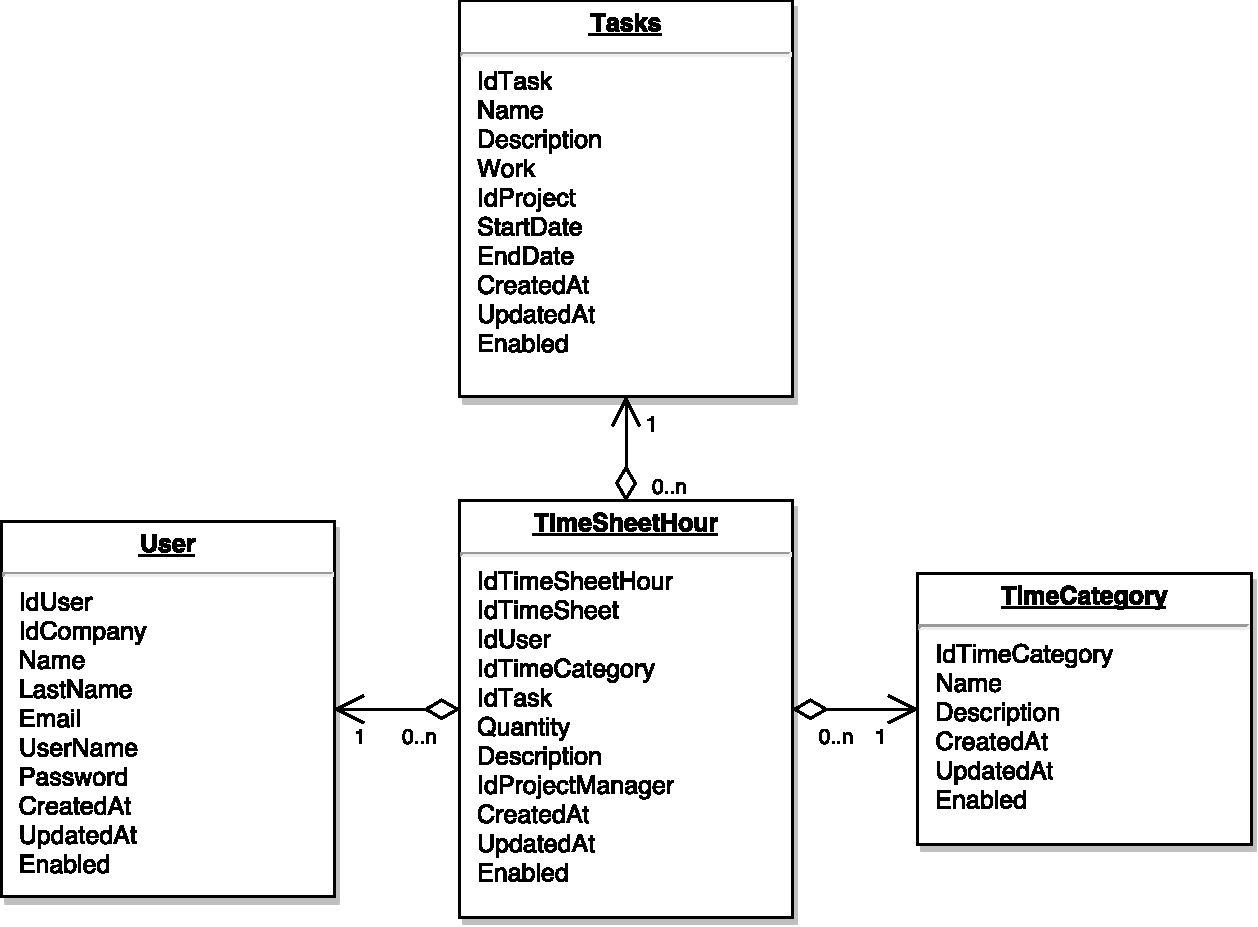
\includegraphics[width=0.8\textwidth]{Bilder/Diagramm.pdf} 
	\caption{Diagramm eines Software Designs}
	\label{fig:Diagramm-DrawIo}
\end{figure}

Ein weiteres kostenloses Tool für die Darstellung von Klassendiagrammen oder auch Sequenzdiagrammen ist \textbf{\href{http://staruml.io/}{StarUML}}. Dieses generiert auch SVG Dateien, welche du mithilfe von Inkscape zu PDF Dateien konvertieren kannst.

%\chapter{Mathematik}

\section{Text}
Hier steht ein beispielhafter Text bei dem nun auf eine sehr bekannte und durchaus vertraute Formel im Text direkt mit $c = \sqrt{a^2 + b^2}$ eingegangen wird. Dabei können auch Winkel wie: $\alpha, \beta, \gamma$ gerne verwendet werden. Weiterhin werden hier nur Formeln im Bereich der $\mathbb{N}$ dargestellt, gerne können diese aber durch Formeln aus diesem Bereich der $\mathbb{R}$ ergänzt werden.

\section{Formeln}
Beachte bei Formeln keine konkreten Werte anzugeben, sondern die Formel stets nur wie in der Literatur nur als Größengleichungen anzugeben.
\begin{align}
	\sum_{n=0}^{\infty}x=b+n\\
	\frac{b*x}{c} = y
\end{align}

Trotz unterschiedlicher Länge kann man die Gleichheitszeichen auf der gleichen Höhe anbringen wie in \autoref{eq:Gleichung1} und \autoref{eq:Gleichung2} dargestellt, zusätzlich kann man diese auch mit Informationen versehen wie in Formel \autoref{eq:Gleichung3} zu sehen.

\begin{align}
	\label{eq:Gleichung1} a + b &= c\\
	\label{eq:Gleichung2} 5c + 3f &= 4h\\ 
	\label{eq:Gleichung3} \overbrace{5y}^{y = 0} + \underbrace{42x}_{x = 1} &= b
\end{align}

\section{Arrays und Matrizen}

\begin{center}
	\(
	\begin{array}{lc|r}
		a&b&c\\
		\hline
		x&y&z\\
		c&a&b
	\end{array}
	\)
\end{center}

\begin{equation}
	\begin{array}{lcl}
		z & = & a \\
		a + b & = & c \\
		f(x,y,z) & = & x + y + z
	\end{array}
\end{equation}

Hier noch ein paar Matrizen Beispiele in \LaTeX{}.

\begin{align}
	\begin{pmatrix}
		a_{11}	& \dots   & a_{1n}\\
		\vdots	& \ddots  & \vdots\\
		a_{n1}	& \dots   & a_{nn}\\
	\end{pmatrix}
	\\[0.4cm]
	\begin{bmatrix} 
		100&250\\
		300&499
	\end{bmatrix}
	\\[0.4cm]
	\begin{Bmatrix} 
		100&250\\
		300&499
	\end{Bmatrix}
	\\[0.4cm]
	\begin{Vmatrix}
		100&250\\
		300&499
	\end{Vmatrix}
\end{align}

\section{Klammern und Kästchen}

\begin{center}
	\( \Vert x\Vert_{p}=
	\left(
	\sum_{i=1}^{n} | x_{i} |^{p}
	\right)^{\frac{1}{p}} \)
\end{center}

\begin{center}
	\( \left.
	\begin{array}{lc|r}
		a&b&c\\
		\hline
		x&y&z\\
		c&a&b
	\end{array}
	\right\}
	\Rightarrow z,b \)
\end{center}

\begin{equation*}
\mbox{
	\boxed{
		\sin^2\varphi+\cos^2\varphi=1
	}
}
\end{equation*}


%\chapter{Programm- bzw. Quellcode}
\section{Quellcode}
Ein wichtiger Punkt ist auch, dass man Quellcode Stücke mit in seinen Praxisbericht einbaut. Hier nun einfach mal ein Beispiel in Form eines kleinen JAVA Codes, welcher aus einer Datei gelesen wird:

\lstinputlisting[
	label=code:algQuersumme,    % Label; genutzt für Referenzen auf dieses Code-Beispiel
	caption=Algorithmus zur Berechnung der Quersumme,
	captionpos=b,               % Position, an der die Caption angezeigt wird t(op) oder b(ottom)
	style=EigenerJavaStyle,     % Eigener Style der vor dem Dokument festgelegt wurde
	firstline=3,                % Zeilennummer im Dokument welche als erste angezeigt wird
	lastline=18                 % Letzte Zeile welche ins LaTeX Dokument übernommen wird
]{Quellcode/Eigenes-Java-File.java}

Zu beachten ist, dass jedes Stück Code kommentiert werden sollte. Was wird in diesem Abschnitt genau durchgeführt. Wo könnten Probleme auftreten und warum wurde dieses Stück hier hinzugefügt.

\vspace*{0.5cm}

\pagebreak
\textbf{EVENT 01} \textit{INIT}
\lstinputlisting[
	label={code:SSCUI-AfterInit},  % Label; genutzt für Referenzen auf dieses Code-Beispiel
	caption={Initialisierung im Programm},
	captionpos=b,               % Position, für die Caption:  t(op) oder b(ottom)
	style=EigenerABAPStyle,     % Eigener Style der vor dem Dokument festgelegt wurde
	firstline=4,                % Zeilennummer im Dokument welche als erste angezeigt wird
	lastline=23                 % Letzte Zeile welche ins LaTeX Dokument übernommen wird
]{Quellcode/Eigenes-ABAP-File.abap}

Es ist auch möglich, innerhalb des Listings \LaTeX{} Befehle zu verwenden. Dazu muss aber eine Escape-Sequenz angegeben werden. Das folgende Beispiel enthält ein Label, auf das dann verwiesen werden wird: Auch hier funktioniert \texttt{\textbackslash{}autoref}: \enquote{In \autoref{code:var_b} wird der Variable \texttt{b} \ldots}.

\begin{lstlisting}[
  style=EigenerJavaStyle,
  captionpos=b,
  caption={Zuweisung von Variablen},
  label={code:basic_block},
  escapeinside={@}{@}]
int a = 10;
@\label{code:var_b}@int b = a + 20;
return;
\end{lstlisting}

\pagebreak
Weitere Programmiersprachen können auch eingebunden werden. Hier mal ein Beispiel in der Programmiersprache Python:
\lstinputlisting[
	label=code:WhileLoop,    % Label; genutzt für Referenzen auf dieses Code-Beispiel
	caption=Algorithmus zum Schätzen einer Zahl in Python,
	captionpos=b,               % Position, an der die Caption angezeigt wird t(op) oder b(ottom)
	style=EigenerPythonStyle,   % Eigener Style der vor dem Dokument festgelegt wurde
	firstline=0,                % Zeilennummer im Dokument welche als erste angezeigt wird
	lastline=23                 % Letzte Zeile welche ins LaTeX Dokument übernommen wird
]{Quellcode/Eigenes-Python-File.py}

\clearpage % Absichtlicher Seitenumbruch, um ein besseres Layout zu erhalten.

\section{Pseudocode}
Pseudocode kann hilfreich sein, wenn \enquote{richtig} implementierte Algorithm in einer Programmiersprache zu lang sind und diese mittels Pseudocode bündig zusammengefasst werden können. \autoref{lst:euclid} zeigt Pseudocode.

Die Doku für das Package und damit eine Liste aller Befehle findet sich unter \newline
\url{http://tug.ctan.org/macros/latex/contrib/algorithmicx/algorithmicx.pdf}

\begin{algorithm}
	\caption{Euclid's algorithm}\label{lst:euclid}
	\begin{algorithmic}[1]
		\Procedure{Euclid}{$a,b$}\Comment{The g.c.d. of a and b}
			\State $r\gets a\bmod b$
			\While{$r\not=0$}\Comment{We have the answer if r is 0}
				\State $a\gets b$
				\State $b\gets r$
				\State $r\gets a\bmod b$
			\EndWhile\label{euclidendwhile}
			\State \textbf{return} $b$\Comment{The gcd is b}
		\EndProcedure
	\end{algorithmic}
\end{algorithm}

%\chapter{Literaturhinweise}

\textbf{Hinweis}: Verwendest du eine Quelle nicht, dann nimmt \LaTeX{} diese nicht mit ins Literaturverzeichnis auf!

\section{Fußnoten und Literaturverweise}
Hamburger, Döner, Currywurst\footnote{Hier fehlt eindeutig das Lieblingsessen der Informatiker, die Pizza!} - jeder kennt sie, jeder liebt sie und jeder isst sie.
Weil die Zeit drängt\cite{Bonnen.2016}, der Hunger groß ist und der nächste Schnellimbiss\cite{Forsthuber.2016} nur drei Schritte voraus. Und nach dem Essen?
Sind wir zwar satt, aber meist nicht wirklich glücklich, weil Fastfood\cite{Friedl.2017} meist eben auch nicht wirklich gut ist \cite{Kuhnlein.2016}.

Ja, uns ist bewusst, dass die Literatur nicht zum Text passt.
Deswegen hier nochmals der Rest.\cite{Mukherjee.2017, Preuss.2017, Schell.2017, Smith.2017, Visser.2017, Zaidi.2017, o.V..o.J.}

Übrigens: \acfp{ISBN} gehören nicht in die Bibliographie und werden deshalb auch nicht angezeigt.


% \chapter{Einleitung}

\section{Motivation und Problemstellung}

Allein in den USA geben Unternehmen jährlich mehr als 200 Milliarden Dollar für Schulungen, Fortbildungen und Seminare aus \parencite[vgl.][]{LloydMewkirk.2011}.
Leider neigen Teilnehmer nach Abschluss jener Veranstaltungen dazu, gelerntes Wissen über die Zeit zu vergessen.
Ein Umstand, der weithin als Vergessenskurve bezeichnet wird und um 1885 vom deutschen Psychologen Hermann Ebbinghaus beschrieben wurde \parencite[vgl.][]{Ebbinghaus.1885}. 

Unternehmen investieren also viele Millionen Dollar in Lernveranstaltungen, nur damit vieles danach wieder in Vergessenheit gerät.
Ein dynamischer Learning-\acs{NFT} versucht dieses Problem nachhaltig, durch anschließende zeitlich versetzte Lerneinheiten zu minimieren und diesen Prozess analysier- und steuerbar zu machen. 
Des Weiteren gibt ein \acf{NFT} die Möglichkeiten verbesserter Fälschungssicherheit und bietet Nutzungsmöglichkeiten auch plattformübergreifend.

\section{Methodik und Vorgehen}

Im ersten Teil der Arbeit sollen die zugrunde liegenden Technologien erklärt und beschrieben werden.
Beginnend mit Grundlagen zur Distributed Leger Technologie und Blockchain soll die Funktionsweise von Smart Contracts erläutert werden.
Auf dieses Gerüst aufbauend werden dann \ac{NFT}s erklärt, sowie eine Abgrenzung zum gern Synonym verwendeten Thema Kryptowährungen vorgenommen werden.

Anschließend sollen Methoden und Ansätze des dynamischen Learning-\ac{NFT}s im Rahmen einer Fallstudie analysiert werden um Potenziale und Adaptionsmöglichkeiten für die Anwendung
auf der SAP Experience Garage Plattform herauszustellen und aufzuzeigen welche Verbesserungsmöglichkeiten die einzelnen Komponenten eines solchen
Learning-\ac{NFT} für die Experience Garage Plattform zukünftig haben könnten und ob sich eine Implementierung des Konzepts im Ganzen,
oder in Teilen, für die SAP Experience Garage lohnt.
Weiterhin könnten spezielle Anforderungen der Plattform eine Erweiterung beziehungsweise Modifikation des Konzepts erfordern beziehungsweise lohnenswert machen.

Abschließend soll nach einer kurzen Auseinandersetzung mit den Schattenseiten der Blockchain Technologie ein Fazit,
zum Adaptionspotenzial eines dynamischen Learning-\ac{NFT}s in die Experience Garage Plattform vorgenommen
und einen Ausblick auf mögliche Anwendung im unternehmensweiten Kontext gegeben werden.

\section{Zielsetzung}

Ziel ist es, die Ansätze und Methoden des Learning-\ac{NFT}s zu analysieren, um Potenziale und Probleme herauszustellen.
Des Weiteren sollen Möglichkeiten zur Adaption eines solchen Konzepts für die Experience Garage Plattform aufgezeigt und bewertet werden.
% \chapter{Grundlagen}

Zu Beginn dieser Arbeit sollen in diesem Kapitel die dem Thema zugrunde liegenden Technologien eingegangen werden, um im Verlauf dieser Arbeit auf dieses Grundverständnis aufbauen zu können.

Zunächst soll auf die technische Basis  eines \ac{NFT}, die Blockchain und die dahinter stehende Distributed-Ledger-Technologie eingegangen werden und die Funktionsweise erläutert werden.
Darauf aufbauend werden Smart Contracts beleuchtet da sie die Implementierung eines NFTs erst ermöglichen.

\section{Blockchain und Distributed-Ledger-Technologie}

Der Begriff Blockchain stammt aus dem Kontext der, oft als Synonym verwendeten, Distributed-Ledger-Technologie, kurz DLT \parencite[vgl.][5]{WILKENS.2019}.

\subsection{Distributed-Ledger-Technologie}

Ins Deutsche übersetzt heißt Distributed Ledger so viel wie verteiltes Kontobuch und bezeichnet eine Netzwerkstruktur in der Daten verteilt organisiert sind (Abb. \ref*{fig:network} rechts).
Die Transaktionshistorie und andere Daten werden bei allen Netzwerkteilnehmern gleichzeitig gespeichert und mithilfe eines Konsensverfahrens verifiziert.
Anders als bei gewöhnlichen Datenbanken (Abb. \ref{fig:network} links) werden die Daten beim \ac{DLT} also weder zentral gespeichert, noch gibt es eine Autorität (Abb. \ref{fig:network} Mitte) welche die Daten verwaltet
\parencite[vgl.][4]{janaessebier.2017}.

    \begin{figure}
        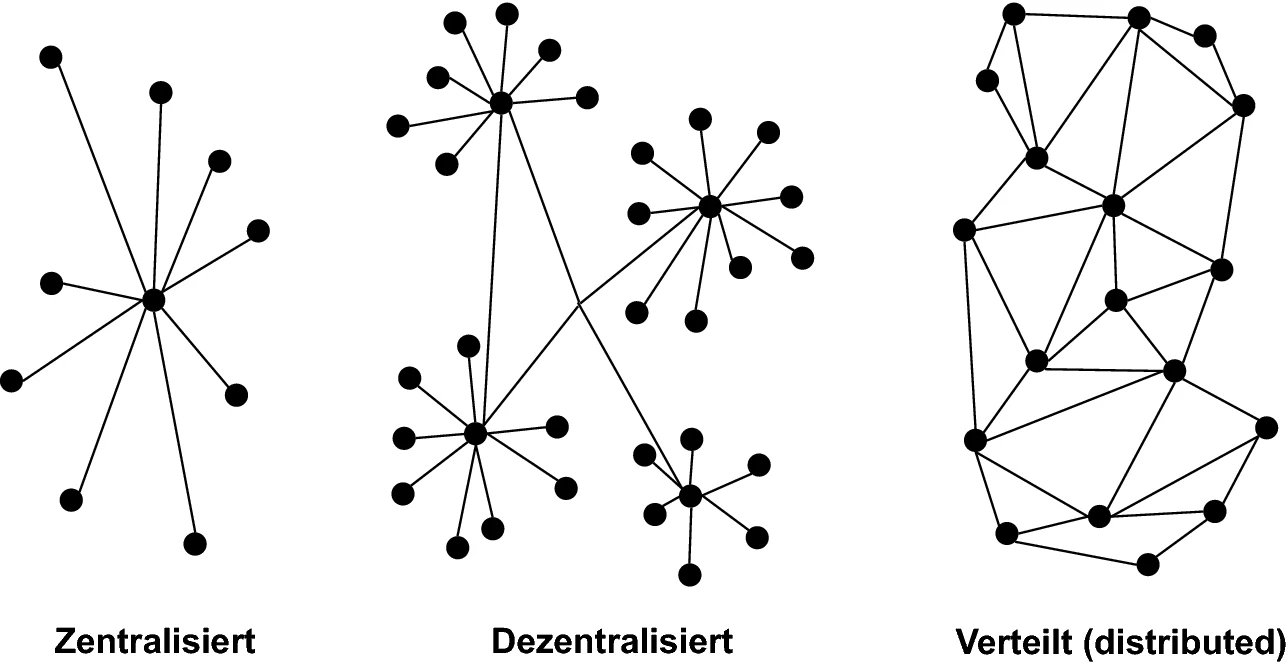
\includegraphics[width=10cm]{Bilder/Netzwerk2 (convert.io).png}
        \centering
        \captionabove[Netzwerktypen]{Netzwerktypen \parencite[vgl.][6]{WILKENS.2019}}
        \label{fig:network}
    \end{figure}

Durch die Verteilung von Datenpflege und transparenter Verwaltung durch eine große Anzahl an Nutzern im Netzwerk sind Daten fälschungssicher und nachvollziehbar.
Ein weiterer Vorteil ist die Unabhängigkeit des Netzwerks vom einzelnen Nutzer, wodurch das System sehr stabil und nahezu ausfallsicher ist \parencite[vgl.][3]{Overcamp.2019}.

\subsection{Blockchain}

Blockchains sind die derzeit bekannteste Ausprägung der \ac{DLT} und spätestens seit der Einführung von Bitcoin sollte jeder diesen Begriff schonmal gehört haben. Aber was ist das besondere an der Technologie?

Die Besonderheit der Blockchain ist die irreversible Speicherung von Transaktionen wie beispielsweise die Überweisung einer Kryptowährung, die Registrierung eines Dokuments oder Vertrags in Form aneinander hängender Blöcke. 

Dafür werden zuerst die zu übermittelnden Transaktionen beim Sender codiert. 
Dann werden die Zeichenfolgen in eine uniforme Codierungen überführt \parencite[vgl.][313]{Neugebauer.2018}.
Diese ist stark kollisionsfrei, es ist also schwer aus verschiedenen Eingaben denselben Wert abzubilden \parencite[vgl.][]{tuchemblockchain}.
Ist die Transaktion dann vom Sender an das Netzwerk übergeben worden und an die Knoten verteilt, beginnt die Prüfung der Transaktion.
Nach einer formalen Prüfung versuchen die Knoten, auch Miner genannt, durch verschiedenste Verfahren wie beispielsweise \ac{PoW} oder \ac{PoS} einen Konsens zu finden.
Zu erläutern wie diese Konsensverfahren funktionieren würde den Rahmen an dieser Arbeit jedoch sprengen. 
Ist der Konsens gefunden, ist die Transaktion validiert und wird mit anderen Transaktionen in einem Block gespeichert.
Dieser Block wird wiederum durch Hashfunktionen in ein standardisiertes Format gebracht und hierarchisch verdichtet.
In den Hashwert ist unter anderem eine Referenz auf den Hashwert des vorigen Blocks integriert, wodurch eine irreversible Verkettung der einzelnen Blöcke entsteht -- die Blockchain.
Das macht die Blockchain-Technologie gegen Manipulationsversuche sicher, weil bereits die Änderung einer einzelnen Transaktion den Hashwert
des gesamten Blocks ändern und damit die Konsistenz des Hash-Baums aufheben würde \parencite[vgl.][313]{Neugebauer.2018}.

    \begin{quote}
        „Diese hierarchische Verdichtung wird als Hash- oder Merkle-Baum bezeichnet, mit dem sich ein Block von Transaktionen eindeutig repräsentieren lässt.“
        \parencite[313]{Neugebauer.2018}
    \end{quote}

    \begin{figure}
        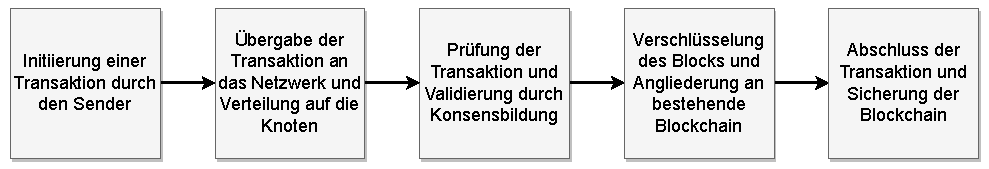
\includegraphics[width=15.8cm]{Bilder/Blockchain_schema.pdf}
        \centering
        \caption{Funktionsweise einer Blockchain}
    \end{figure}

Um die Blockchain persistent zu sichern wird die gesamte Blockchain in jedem Knoten gespeichert und bei jedem neuen Block erweitert.
Die Blockchain Technologie könnte man also als eine Art verteilte von Nutzern verwaltete Datenbank sehen.
Diese verteilte Datensicherung und -verarbeitung ist gegenüber zentralen Ansätzen deutlich weniger fehleranfällig,
bringt jedoch auch einen hohen Verbrauch an Ressourcen wie Speicherplatz und Stromverbrauch mit sich \parencite[vgl.][314]{Neugebauer.2018}.

\section{Smart Contracts}

Die Herkunft des Begriffs Smart Contract geht auf den amerikanischen Informatiker und Juristen Nick Szabo zurück,
welcher erstmals ende der 90er Jahre das Konzept rechtsrelevanter Computerprogramme und -protokolle beschrieb.

    \begin{quote} 
        „Ein Smart Contract ist eine Reihe von Zusagen, die in digitaler Form niedergelegt werden, einschließlich Protokollen, in denen die Parteien diese Zusagen einhalten.“
        \parencite[3]{WILKENS.2019}

        „[…] A smart contract is a set of promises, specifed in digital form, including protocols within which the parties perform on these promises.“
        \parencite[]{.23.01.2006}
    \end{quote}

Nick Szabo nutze für Erklärungen das Beispiel eines Warenautomats: Der Kunde wirft genügend Geld in den Automaten wählt das gewünschte Produkt und bekommt es ausgeworfen.
Im Gegenteil zum Supermarkt ist hier keine andere Person unmittelbar beteiligt und der Kauf findet automatisiert statt.
Ebenso funktionieren Smart Contracts auf digitaler Ebene, wie beispielsweise in Abbildung \ref{smartcontract} \parencite[vgl.][618]{Kaulartz.2016}:

    \begin{enumerate}
        \item Prüfbares Ereignis wird digital ausgelöst (Eingang der Transaktion)
        \item Programmcode verarbeitet das Ereignis (Prüfung der Transaktion)
        \item Handlung auf dessen Grundlage das Ereignis wird ausgeführt (Ausgabe der Ware)
    \end{enumerate}

Die Smart Contracts agieren dabei komplett automatisch und bringen damit ein hohes Potenzial für den digitalen Geschäftsverkehr mit,
da viele Prozesse automatisiert werden könnten \parencite[vgl.][27]{JohannesScherk.2017}.

Aber die Möglichkeit der Automatisierung ist nicht der alleinige Grund für die steigende Euphorie gegenüber Smart Contracts.
Die wichtigste Bedeutung entsteht in Verbindung mit der Blockchain-Technologie.
Hier können die Smart Contracts in manipulationssicheren Datenstrukturen und in redundanter Form auf allen Miner-Instanzen des Netzwerks gesichert werden.
Womit sie das komplette Gegenteil des bisher genutzten Client-Server-Modells darstellt.

Die erste Anwendung dieser Technologie ist heute allgemein hin als die Kryptowährung Bitcoin bekannt.
Durch eine Weiterentwicklung des Konzepts ist es auch möglich Programmcode in der Blockchain abzulegen und auszuführen.
Diese komplett autonomen Akteure innerhalb des Netzwerks, werden allein durch ihren Code gesteuert und ermöglichen es damit zuvor festgelegte Prozesse innerhalb der Blockchain-Umgebung automatisiert auszuführen.
Heutzutage werden mit dem Begriff Smart Contracts deshalb in aller Regel kleine Programme auf der Blockchain bezeichnet \parencite[vgl.][4]{WILKENS.2019}.
Folgende Definition wird festgehalten:

    \begin{quote}
        „Als Smart Contracts werden Programme auf der Blockchain bezeichnet, die auf Basis einer WENN-DANN-Logik arbeiten, 
        sodass bei Eintritt eines zuvor festgelegten Ereignisses (sog. Trigger)
        automatisch eine ebenfalls zuvor festgelegte Aktion (bspw. eine Transaktion) ausgeführt wird.“
        \parencite[4]{WILKENS.2019}
    \end{quote}

    \begin{figure}
        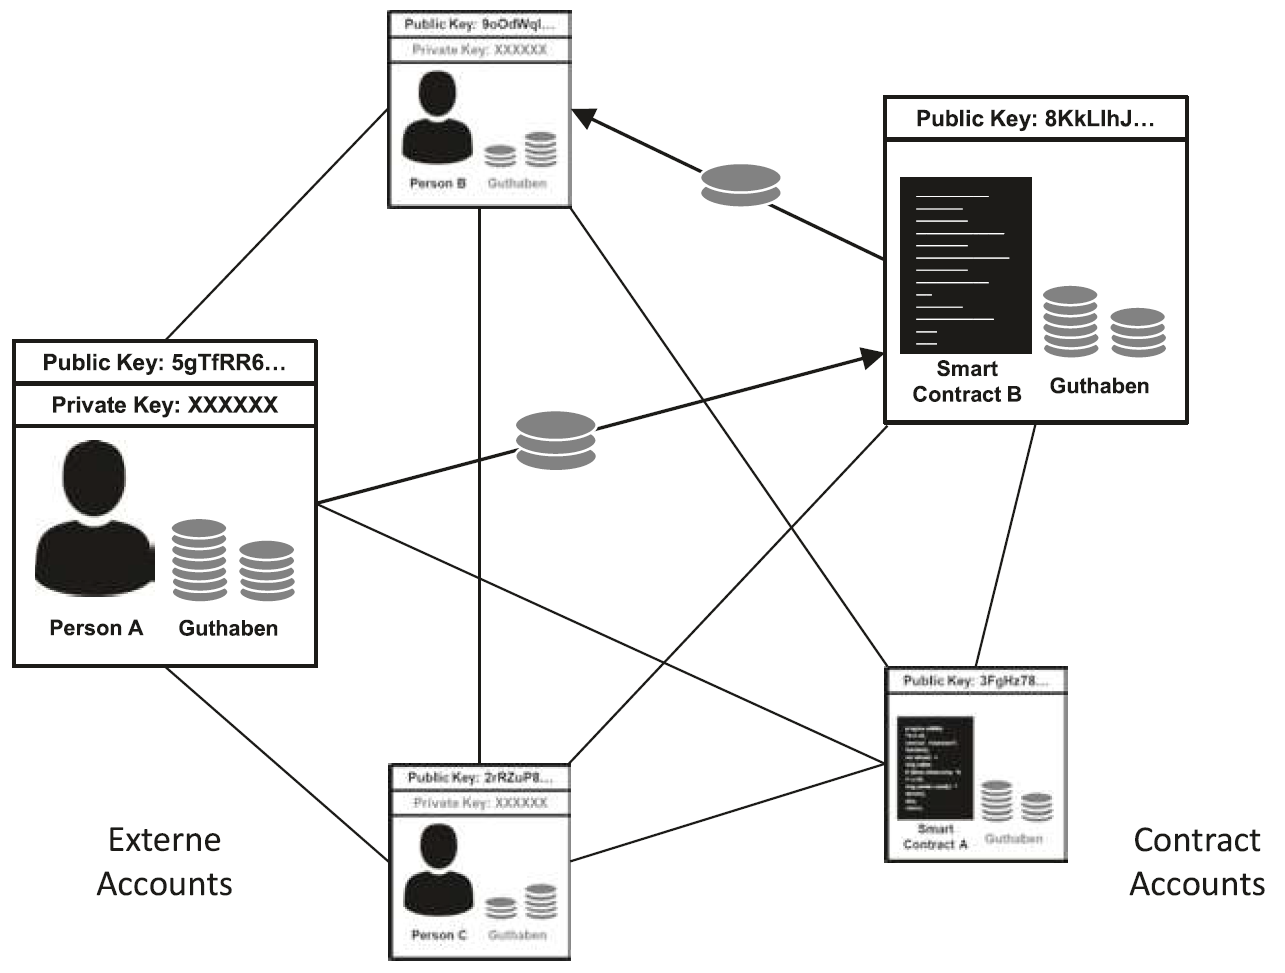
\includegraphics[width=12cm]{Bilder/Smart Contracts.PNG}
        \centering
        \captionabove[Interaktion zwischen Personen und Smart Contracts]{Interaktion zwischen Personen und Smart Contracts \parencite[vgl.][11]{WILKENS.2019}}
        \label{smartcontract}
    \end{figure}

\section{NFTs vs Kryptowährungen}

Da die technischen Grundlagen nun dargestellt wurden, soll nun erklärt werden was einen \ac{NFT} ausmacht und wo die Unterschiede zu, oft direkt im Zusammenhang genannten, Kryptowährungen bestehen.
Gemein haben \acl{NFT}s wie auch Kryptowährungen die zugrundeliegende Blockchain-Technologie und werden über Kryptobörsen veräußert.
Um die Unterschiede besser darstellen zu können wird kurz erklärt, was eine klassische Kryptowährung spezifiziert \parencite[vgl.][13]{BenjaminKraudinger.2022}.

Kryptowährungen wie beispielsweise Bitcoin, Ether (Währung der Ethereum-Blockchain) und Binance Coin sind durch zwei Charakterstika gekennzeichnet:

Zunächst wird eine Kryptowährung von Beginn an in der Blockchain implementiert.
Es ist also von Anfang an im Quellcode festgelegt welche Bezeichnung und weiteren Eigenschaften die Währung besitzt. 
Wenn sogenannte \dq Miner\dq{} also neue Einheiten erschaffen ist das eher irreführend da diese bereits im Programm vorgesehen waren und unter bestimmten Voraussetzungen freigeschaltet werden \parencite[vgl.][801]{Gassebner.2018}.
Bei Bitcoin sind das zum Beispiel maximal 21 Millionen Bitcoin \parencite[vgl.][76]{Segendorf.2014}.

Zum anderen ist der Hauptzweck von Kryptowährungen die Benutzung als Zahlungsmittel, weshalb Kryptowährungen auch als \ac{PT} bezeichnet werden \parencite[vgl.][924]{Max.2021}.
Um dies zu erreichen, dürfen sich Token zum Beispiel ein Bitcoin, nicht im Wert von einem anderen unterscheiden, im Englischen als fungibility bezeichnet \parencite[vgl.][7]{Fairfield.2021}.

Diese beiden Eigenschaften hat ein \ac{NFT} nicht. Einerseits ist ein \ac{NFT} nicht von vornherein in der Blockchain verankert,
sondern wird durch die im Grundlagenkapitel bereits erläuterten Smart Contracts an die Blockchain angefügt.
Zum anderen sollen sie nicht als Zahlungsmittel eingesetzt werden und können daher jeden beliebigen Wert annehmen.

Ein \ac{NFT} bietet die Möglichkeit auf moderne Art digitale Werteträger auf Blockchain Basis darzustellen.
Wie im Namen schon enthalten handelt es sich dabei um nicht vertretbare Token.
Besonders daran ist, dass sie einzeln vollkommen individuell sind und es prinzipiell keinen gleichen Token gibt,
letztendlich also \dq digital Einzigartig\dq{} ist \parencite[vgl.][13]{Fairfield.2021}. 

Damit bietet ein \ac{NFT} die Lösung eines bisher großen Problems im digitalen Raum:
Digitale Werte, reichend von Abbildungen von berühmten Gemälden, bis hin zu limitierten Ausrüstungsgegenständen in Computerspielen,
einem Besitzer zuordnen und zertifizieren zu können.
Denn bisher konnten diese Werte mit minimalem Aufwand verlustfrei kopiert werden,
ohne Original und Kopie im Nachhinein unterscheiden zu können. Damit ist es auch schwer möglich einen \dq wahren\dq{} Besitzer zuzuordnen \parencite[vgl.][13]{Fairfield.2021}.

Ein \ac{NFT} kann dieses Problem lösen in dem der Token ein Objekt, beispielsweise ein Kunstwerk,
auf der Blockchain repräsentiert dem eine Seltenheit zugewiesen werden soll.
Das digitale Gut wird dabei in der Regel nicht direkt in die Blockchain aufgenommen (Off-Chain \ac{NFT}).
Es enthält lediglich eine Referenz auf den Speicherort,
sowie ein Hash der Datei des Guts um die Verbindung von Gut und \ac{NFT} beweisen zu können \parencite[vgl.][23]{Fairfield.2021}.
Eine andere Möglichkeit, On-Chain \ac{NFT} genannt, sieht vor das die Datei unmittelbar in der Blockchain verankert wird.
Prinzipiell sind diese Dateien deshalb jedoch deutlich größer und je größer die auf die Blockchain zu übertragende Datenmenge,
desto höhere Transaktionsgebühren sind zu zahlen.

Wird also beispielsweise ein digitales Kunstwerk von Person A durch einen \ac{NFT} repräsentiert und an Person B verkauft,
ändert sich der Speicherort des Bildes nicht, der \ac{NFT} wechselt jedoch seinen Besitzer.
Angenommen eine dritte Person würde sich Zugang zum Speicherort des Kunstwerks verschaffen und die Datei kopieren, so wäre die Datei an sich dieselbe,
könnte jedoch als Raubkopie leicht enttarnt werden,
da in der Blockchain zu erkennen ist, dass sich das Kunstwerk erst im Besitz von A befand und dann in dem Besitz von Person B überging.
Nur Person B ist also rechtmäßiger Eigentümer des Kunstwerks und hat alleinige Verfügung.
Wie bereits beschrieben kann man diese Transaktionen im Nachhinein nicht mehr verändern oder verfälschen.
Die Blockchain kann also durch \ac{NFT} Anwendung auch zu einem Register für Besitzerstellungen sein \parencite[vgl.][567]{Hoeren.2021}.
% \chapter{Fallstudie Dynamische Learning-NFTs}

In diesem Kapitel wird das Konzept eines Learning \ac{NFT}s im Rahmen einer Fallstudie analysiert und erläutert.
Basis der Analyse bietet hierbei der von Peter C. Evans entwickelte MyLearning\ac{NFT} \parencite[vgl.][]{MyLearningNFT.2022}.
Nach Erläuterung der Funktionsweise sollen verbesserte Einflussmöglichkeiten auf einen nachhaltigen Lernprozess aufgezeigt werden und wie diese Daten Institutionen helfen können.
Dann wird auf die Besonderheit eines dynamischen \ac{NFT} eingegangen und welche Vorteile die Blockchain bezüglich Fälschungssicherheit, Transparenz und Plattformunabhängigkeit bieten kann.
Abschließend wird zudem der Trend um \ac{NFT}s und Blockchain näher beleuchtet. 

\section{Funktionsweise}

Der dynamische MyLearning\ac{NFT} ändert seinen Status, je nachdem wie der Teilnehmer nach einer abgeschlossenen Schulung oder Fortbildung weiterlernt.
Dabei gibt es zwei Hauptaspekte:
Zum einen gibt es Lernaktivitäten die bezeichnen wie der Teilnehmer lernt,
beispielsweise durch Lesen eines Artikels oder das Hören eines Podcasts.
Zum anderen die Wissensbereiche, also die Themen, die ein Teilnehmer im Anschluss an ein Lernevent weiter vertiefen und lernen soll.
Diese Daten werden bereits vor Beginn des Kurses durch den Veranstalter vorbereitet
und können nach dem Event über den Account eines jeden Nutzers auf der Webseite eingetragen werden und müssen dann vom Veranstalter validiert werden.
Der Nutzer bekommt für die Lernaktivität dann eine bestimmte Anzahl von Punkten gutgeschrieben, welche wiederum den Score verändert und eine Einteilung in 5 Stufen ermöglicht, siehe Abbildung \ref{stufen} \parencite[vgl.][]{MyLearningNFT.2022}.

\begin{figure}[ht]
    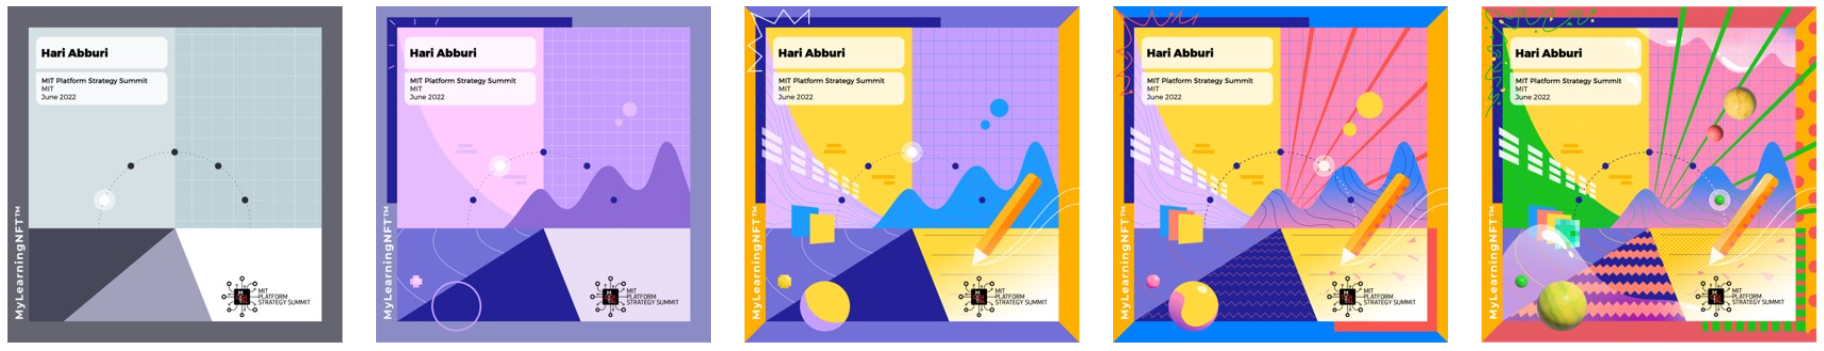
\includegraphics[width=15.8cm]{Bilder/Stufen.PNG}
    \centering
    \captionabove[Stufen 1-5 des MyLearningNFT]{Stufen 1-5 des MyLearning\ac{NFT} \parencite[vgl.][]{MyLearningNFT.2022}}
    \label{stufen}
\end{figure}

Direkt nach dem Event startet der Teilnehmer mit 50 Punkten, was der mittleren Stufe entspricht.
Lernt ein Teilnehmer innerhalb von 90 Tagen nach einem Lernevent weiter und sammelt Punkte, so behält der \ac{NFT} seinen Status oder erhöht sich.
Bleibt der Teilnehmer nach dem Event nicht an dem Thema dran und macht keine Auffrischungen, weiterführende Lerneinheiten o.ä. wird davon ausgegangen,
dass der Teilnehmer, wie von Ebbinghaus beschrieben, Stück für Stück mehr des gelernten wieder vergisst.
Beim \ac{NFT} sinkt dann über die Zeit das Punktekonto und der \ac{NFT} ändert den Status negativ \parencite[vgl.][]{MyLearningNFT.2022}.

\section{Nachhaltiges Lernen}

Um den Status des \ac{NFT} auf einer hohen Stufe zu halten, muss sich der Teilnehmer immer wieder aktiv mit dem Thema Auseinandersetzen.
Diese Lernmethode der Wiederholung sorgt dafür, dass erlerntes Wissen nachhaltiger gespeichert und zu einem späteren Zeitpunkt wieder abgerufen werden kann \parencite[vgl.][221-223]{Sattler.2009}
und wirkt der Vergessenskurve nach Ebbinghaus damit entgegen.
Der Teilnehmer kann einen deutlich größeren Anteil der Inhalte über einen längeren Zeitraum behalten und erworbenes Wissen nachhaltig eingesetzt werden.
Der Wert der Lernaktivität ist damit über einen längeren Zeitraum gesehen um einiges höher (siehe Abbildung \ref{forg}).

\begin{figure}[h]
    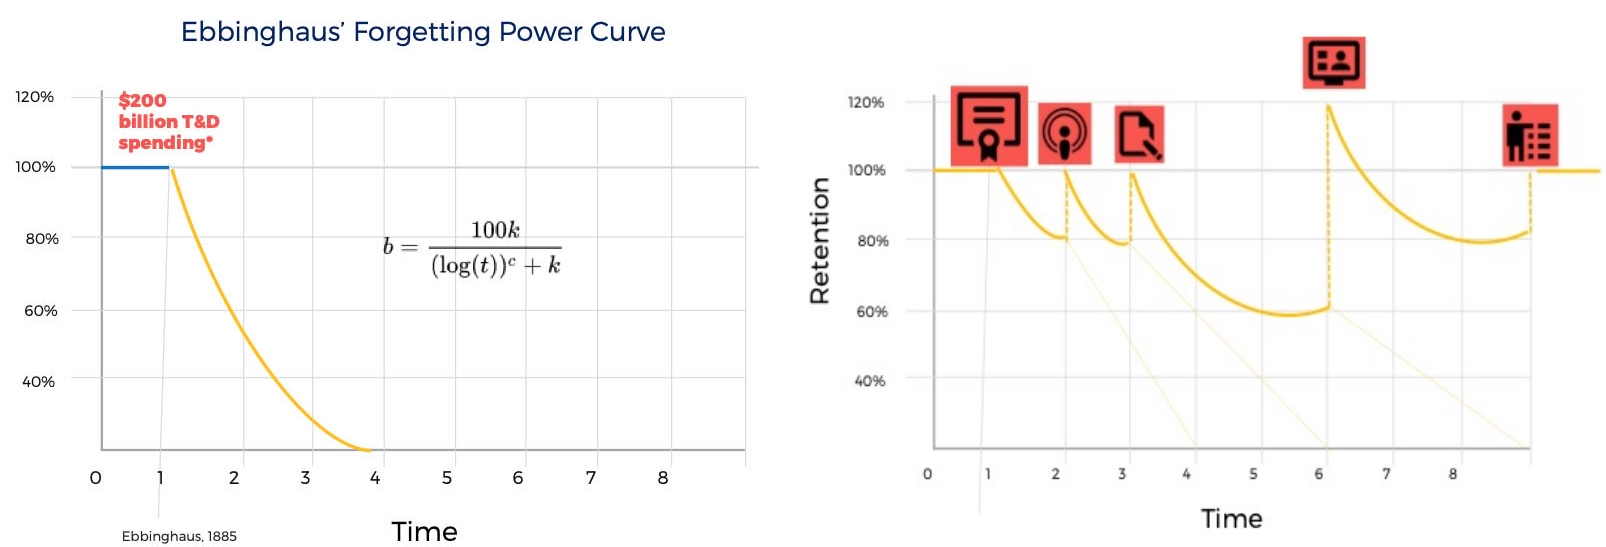
\includegraphics[width=15.8cm]{Bilder/EbinghausForgeting.png}
    \centering
    \captionabove[Vergessenskurve mit Verwendung des MyLearningNFT]{Vergessenskurve normal (links) und mit beispielhafter Verwendung des MyLearning\ac{NFT} (rechts) \parencite[vgl.][]{MyLearningNFT.2022}}
    \label{forg}
\end{figure}

Verknüpfungen von Schulungen und Fortbildungen mit dem MyLearning\ac{NFT} können einen großen Einfluss auf nachhaltiges Verinnerlichen der Inhalte haben.
Eine, im Vergleich zum Lernevent, kleine zusätzliche Investitionen von 1\% bis 3\% in einen Learning \ac{NFT} kann die Effektivität des Events damit erheblich steigern
und ist auch aus ökonomischer Sicht sehr sinnvoll \parencite[vgl.][]{MyLearningNFT.2022}.

\section{Datenerhebung zum Lernverhalten}

Der Mangel an Daten zum Lernverhalten ist ein weiteres Problem das gelöst werden kann.
Institutionen und Unternehmen können kaum Daten über das Lernverhalten der Teilnehmer nach einem Kurs oder Seminar sammeln
oder wie sie sich über den Kurs hinaus weiter mit dem Thema beschäftigen und weiter lernen.
Das Analysetool des MyLearning\ac{NFT} kann Unternehmen dabei helfen zu verstehen wie die Teilnehmer nach dem Event lernen und in welchen Themengebieten.
Mit diesen Informationen kann Veranstaltern und Unternehmen geholfen werden zukünftige Schulungen und Seminare besser anzupassen und ausrichten zu können.
Die Vorteile liegen klar auf der Hand:
Das Event kann für den Teilnehmer effektiver gestaltet werden.
Zum anderen kann das Ereignis der Investition in Lerneinheiten und Entwicklungsprogramme erheblich gesteigert werden \parencite[vgl.][]{MyLearningNFT.2022}.

\section{Dynamische NFTs}

Im Grundlagenkapitel wurde bereits erklärt wie basierend auf der Blockchain in Verbindung mit Smart Contracts ein \ac{NFT} funktioniert.
Ein dynamischer \ac{NFT} stellt wiederum eine kleine Besonderheit dar.
Denn \dq normale\dq{} \ac{NFT}s, wie zum Beispiel das Besitzzertifikat für ein digitales Kunstwerk, sind statisch und können nicht verändert werden.
Durch die Einführung von Layer-2-Skalierung ist es aber möglich geworden spezifische Tokens zu erstellen,
die mit der Blockchain verknüpft sind und durch bestimmte Events geändert werden können.
Realisiert wird das durch die Einführung von Side-Chains, welche mit dem Hauptzweig verbunden sind.
Diese Child-Blockchains oder auch Plasma-Blockchains speichern gelegentlich einen Fingerabdruck der Plasma-Chain auf die Root-Blockchain \parencite[vgl.][]{BitcoinSuisse.2020}.
Im Fall vom MyLearning\ac{NFT} wäre das die Ethereum-Blockchain \parencite[vgl.][]{MyLearningNFT.2022}.
Die Reduzierung der Daten für die Root-Chain verkürzt Transaktionen und spart damit Kosten.
Auch kann das Konsensverfahren auf der Plasma-Chain angepasst und spezifisch an die Anforderungen des dynamischen \ac{NFT} angepasst werden \parencite[vgl.][]{BitcoinSuisse.2020}.

Den \ac{NFT} in seinem Wert dynamisch anpassen zu können ermöglicht das \dq Wissenslevel\dq{} des Teilnehmers aktuell darzustellen.
Herkömmliche gamifizierte Lernplattformen wie die aktuelle SAP Experience Garage Technology Plattform arbeiten mit dem Prinzip eines sich nur positiv ändernden Score der immer weiter steigt.
%Ein solch steigender Score motiviert den Mitarbeiter zwar in erster Hinsicht mehr, weil er einen ständigen Anstieg seiner Punkte sieht.
Aussagekraft über sein \dq Wissenslevel\dq{} hat der Wert jedoch kaum.

Angenommen ein Benutzer hat vor vier Jahren einen Python-Workshop mitgemacht, fünf Lerneinheiten abgeschlossen und an zwei Projekten mitgearbeitet.
Danach hat er bis heute, über einen Zeitraum von drei Jahren, keine Berührung mehr mit der Programmiersprache gehabt.
Den Score, den er dafür vor drei Jahren bekam, hat heute immer noch denselben Punkte-Wert. 
Aktualität hat dieser jedoch Wert nicht mehr, ebenso wenig eine sinnvolle Vergleichbarkeit oder sichtbare Qualifizierungsmöglichkeit.
Denn die Programmiersprache hat sich weiter entwickelt und der Teilnehmer hat viel des gelernten vergessen und ist nicht mehr abrufbar, siehe Abbildung \ref{forg}.
Ein Score, der das aktuelle \dq Wissenslevel\dq{} des Teilnehmers widerspiegelt, hätte für Nutzer daher eine deutlich höhere Relevanz und könnte für bessere Vergleichbarkeit der Teilnehmer sorgen,
als auch eine Möglichkeit bieten, Teilnehmer ein aktuelles Skill-Level zu bescheinigen beziehungsweise zertifizieren zu können.

\section{Fälschungssicherheit und Transparenz} \label{fundt}

Einen zusätzlichen Gewinn für den Benutzer stellt die Fälschungssicherheit und Transparenz dar.
Für Fälschungssicherheit sorgt die ständige Protokollierung der Transaktionen in der Blockchain, durch welche es nicht mehr möglich ist eine Transaktion nachträglich zu manipulieren.
Transparenz entsteht durch die Öffentlichkeit der Blockchain, welche die Möglichkeit bietet, alle Transaktionen zurückverfolgen und prüfen zu können \parencite[vgl.][13]{WILKENS.2019}.

Der Nutzer eines MyLearning\ac{NFT} kann also sicher sein das seine Daten manipulationssicher gespeichert sind und geben ihm ein hohes Sicherheitsgefühl und Vertrauen in den Learning-\ac{NFT}.

\section{Plattformunabhängigkeit}

Dass der Learning-\ac{NFT} in einer öffentlichen Blockchain gesichert ist, macht ihn das zudem Plattformunabhängig.
Zum einen hat das den Vorteil, dass wenn die Ursprünglich genutzte Plattform abgeschaltet wird,
der Learning-\ac{NFT} weiter existieren und dank Smart Contracts auch weiterhin mit neuen Daten gefüttert werden kann.
Zum anderen kann der \ac{NFT} auch von anderen Plattformen durch die Smart Contracts genutzt werden.

Diese Plattformunabhängigkeit zusammen mit den bereits erwähnten Vorteilen bezüglich Fälschungssicherheit und Transparenz
eines Learning-\ac{NFT} schafft ein großes Potenzial dem Learning-\ac{NFT} eine weitreichendere Wirkung zu verleihen
und ein aussagekräftiges \dq Wissenslevel\dq{} des Teilnehmers in verschiedenen Kategorien bereitzustellen.
Der Learning-\ac{NFT} könnte hier eine neue sichere und immer aktuelle Möglichkeit eines Lernzertifikats darstellen.

\section{Blockchain und NFTs: Hype oder Zukunft}

Nicht zu unterschätzen ist in Bezug auf \ac{DLT}, Blockchain und \ac{NFT}s auch der Einfluss des Hypes um die Technologien.
Kaum ein Markt ist in den letzten Jahren so gewachsen wie diese.
Allein \ac{NFT}s sind mit einem Handelsvolumen von 2 Milliarden USD im ersten Quartal 2021 auf 16,5 Milliarden USD ein Jahr später gestiegen.
Auch die Anzahl an Krypto-Wallets ist in diesem Zeitraum explodiert und hat sich verzehnfacht \parencite[vgl.][]{NonFungible.2022}.
Der Marktbericht von Verified Market Research geht sogar davon aus das die Branche bis 2030 durchschnittlich um 33,7\% jährlich wächst und auf ein Volumen von 231 Milliarden USD ansteigt \parencite[vgl.][]{VerifiedMarketResearch.2022}.
Ähnliche Prognosen gibt auch SkyQuest ab \parencite[vgl.][]{Skyquest.2022}.

Auch in der Öffentlichkeit sind Blockchain und \ac{NFT}s immer mehr ein Begriff \parencite[vgl.][]{PSW.2022}.
Blockchain hat ein gutes Image und wird als sicherer Ort für revisionssichere Speicherung gesehen.
Bei \ac{NFT}s gehen die Meinungen etwas weiter auseinander.
Technisch weniger versierte Menschen sind verwirrt, warum man digitale Bilder und Accessoires als einen \ac{NFT} kauft und was man überhaupt damit machen sollte.
Menschen, die sich mit dem Thema beschäftigt haben oder sich im Bereich neuer Technologien bewegen, können damit schon mehr anfangen und sehen große Potenziale und welchen Nutzen NFTs mit sich bringen \parencite[vgl.][]{vparthier.23.04.2022}.

Ein Lernzertifikat als einen \ac{NFT} ausgestellt zu bekommen ruft dabei für den Benutzer ein innovatives und sicheres Gefühl hervor und strahlt einen hohen Wert aus.
Diese positive Wahrnehmung wirkt sich wiederum vorteilhaft auf die Lernaktivität aus und hilft bei der Anerkennung und Verbreitung des Learning-\ac{NFT}. 


% \include{Inhalt/04_Inhalt/anwendbarkeitfürXGP.tex}
% \chapter{Schlussbetrachtung}

\section{Kritische Reflektion}

Neben den vielen Potenzialen eines dynamischen Learning-NFT und der darunter liegenden Blockchain Technologie gibt es jedoch auch Schattenseiten.

Der Energiekonsum der Blockchain Technologie ist seit seiner Entstehung ein heiß diskutiertes Thema.
Denn für die Transaktionsprüfung sind spezifische kryptografische Probleme zu lösen.
Diese Hashes werden von \dq Minern\dq{} mit speziell designten Computern rund um die Uhr berechnet, was jedoch viele reale Ressourcen wie Rechenleistung und Energie benötigt \parencite[vgl.][]{Cvj.ch.01.04.2022}.
So hat zum Beispiel die Bitcoin Blockchain mit über 5 Millionen Hardwaregeräten einen jährlichen Stromverbrauch von 89 \ac{TWh}.
Klingt erstmal viel, im Vergleich zum weltweiten Energiebedarf von 162.194 \ac{TWh} ist es aber ein lediglich geringer Anteil von 0,05\% \parencite[vgl.][11]{CoinShares.2022}.

Trotz dessen ist es immer noch ein hoher Verbrauch und verursacht jährlich 36 \ac{Mt} CO\textsubscript{2}.
Immer effizienter werdende Computersysteme können den Stromverbrauch und damit auch die CO\textsubscript{2} Emissionen verringern
(siehe Abbildung \ref*{fig:btceff}) haben aber leider nur einen geringen Einfluss.

    \begin{figure}
        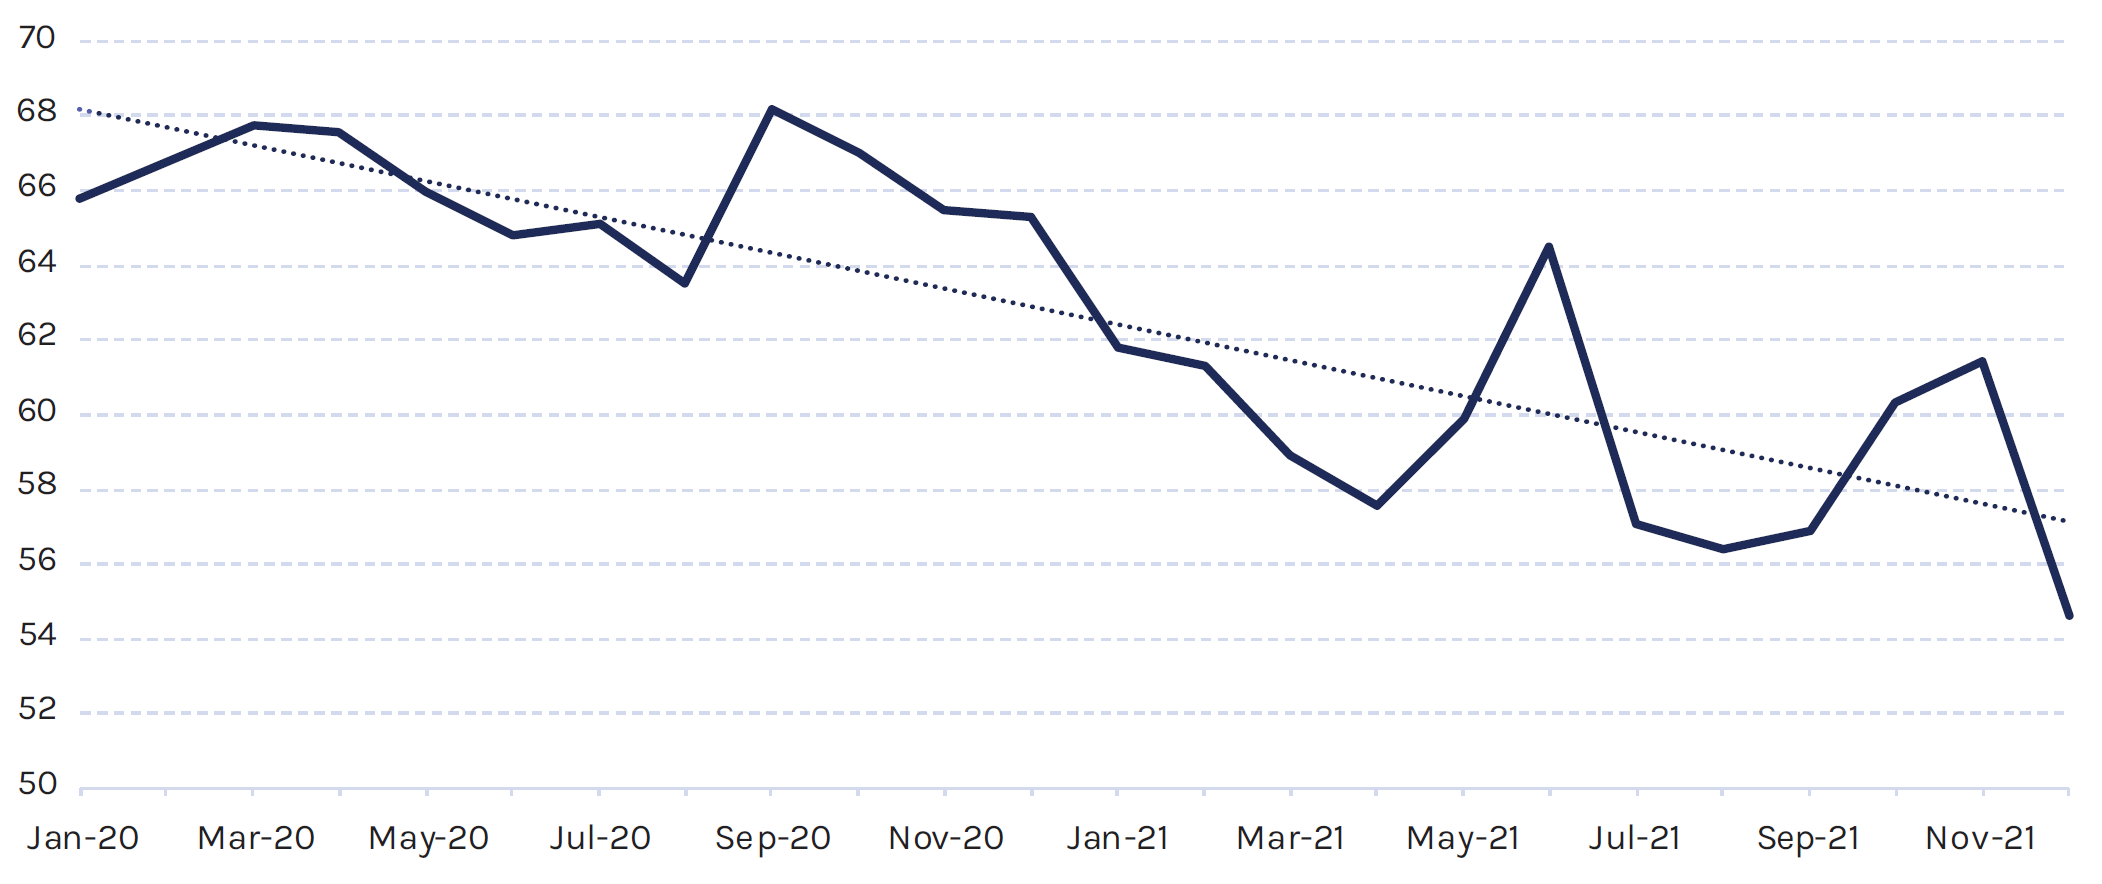
\includegraphics[width=15.8cm]{Bilder/BitcoinEffizienz.PNG}
        \centering
        \captionabove[Effizienz des Bitcoinnetzwerk]{Zeitlicher Verlauf der Effizienz des Bitcoinnetzwerk in Joule pro Tera-Hash \parencite[vgl.][]{CoinShares.2022}}
        \label{fig:btceff}
    \end{figure}

Der hohe Verbrauch der Bitcoin Blockchain ist dabei vor allem auf die Art des Einigungsverfahrens zurückzuführen.
Denn Blockchain arbeitet, wie schon im Grundlagenkapitel erwähnt, mit dem \acf{PoW}, also \dq Beweis durch Arbeit\dq{}.
Eben jene Arbeit ist für den größten Teil des Energiebedarfs zuständig.
Die Blockchain Ether möchte deshalb mit Ethereum 2.0 sein Konsensverfahren von \ac{PoW} auf \acf{PoS} umstellen.
Dieser Prozess ist nicht auf viel Rechenleistung und Energie angewiesen und könnte damit eine grünere Blockchain ermöglichen.
Leider ist bei \ac{PoS} gegenüber \acf{PoW} durch dieses verfahren auch die Manipulation etwas weniger aufwändig und damit ein wenig unsicherer \parencite[vgl.][]{Ginsburg.10.11.2021}.

\section{Fazit}

Abschließend lässt sich sagen, ein Learning-NFT ist ein vielversprechendes Konzept und bietet neue Möglichkeiten nachhaltiges Lernen in verschiedensten Formen zu verbessern, erweitern und steuern zu können.
Für die SAP Experience Garage Technology Plattform ist das Konzept auch sehr interessant, den dynamischen Learning-NFT aber komplett mit allen Bestandteilen umzusetzen ist jedoch nicht sinnvoll.
Wie in Kapitel \ref{testref} beschrieben würde die Implementierung der Methodik und Funktionsweise zum Lernen durch wiederholte Lerneinheiten, in Verknüpfung mit einem Score,
einen großen Wert für Plattform und Nutzer bei geringem Implementierungsaufwand bieten.
Diesen Score in einem NFT abzulegen würde jedoch kaum Nutzen bringen und hohen Zeitaufwand als auch hohe monetäre Kosten für Transaktionen verursachen. 

\section{Ausblick}

Das Konzept von dynamischen Learning-NFTs ist noch in seiner Anfangsphase.
Für die Zukunft lässt sich aber nach Betrachtung dieser Arbeit sagen, dass die Potenziale des Learning-NFTs sehr groß sind und Abseits von der SAP Experience Garage Technology Plattform noch einen deutlich größeren Mehrwert liefern können.
Eine Anwendung wie beispielsweise SAP SuccessFactors \parencite[]{SAP.28.08.2022} oder LinkedIn.

\chapter{Einleitung}

\section{Unternehmensprofil und Anwendungsbezug}

SAP SE ist ein börsennotierter Softwarekonzern mit Sitz in Walldorf. Das Hauptgeschäft des 1972 gegründeten Unternehmens ist die Entwicklung von Unternehmenssoftware zur Abwicklung von Geschäftsprozessen. Heute erwirtschaften 105.000 Mitarbeiter in 157 Ländern einen Umsatz von ca. 30 Mrd. \euro{}. Erfolgreich wurde das Unternehmen mit dem Verkauf von ERP Standardsoftware. In den letzten Jahren stand die Transformation des gesamten Produkt-Portfolios in Richtung Cloud-Services als Abo-Modell im Fokus der Unternehmensstrategie. \footcite[Vgl.][]{sap_geschichte_2023}

Die Abteilung AIS HCM ist Teil des Unternehmensbereichs Product Engineering und zuständig für 2nd-Level-Support und Eigenentwicklungen der SAP Personallösung HCM. Zudem stellt die Abteilung mehrere SAP Fiori Apps als Self-Service für Mitarbeiter bereit. Durch das hohe Nutzungsvolumen dieser Apps und der somit gro{\ss}en betriebswirtschaftlichen Relevanz, sind diese und auch der Untersuchungsgegenstand dieser Arbeit für das Produkt HCM von gro{\ss}er Bedeutung.

\section{Motivation und Problemstellung}

Im folgenden Kapitel soll dargestellt werden, welche Probleme sich durch gewisse technische Veränderungen der SAP Produkte ergeben und sich somit für eine wissenschaftliche Untersuchung im Rahmen dieser Arbeit anbieten.

Die von der Abteilung betriebenen Fiori Apps, die schon im Zusammenhang der Einleitung angesprochen wurden, sind auf Basis des Frameworks SAP UI5 Freestyle für ein älteres Produkt - SAP ERP - entwickelt worden. Durch die strategische Entscheidung HCM im neuen S/4 HANA System (''S/4'' abgekürzt) durch die neue cloudbasierte Personallösung SuccessFactors abzulösen war dieser Umstand ursprünglich kein Problem. Diese Entscheidung wurde aufgrund fehlender Funktionalitäten in SuccessFactors und hoher verlässlicher Einnahmen durch Wartungsverträge für HCM revidiert und HCM ist Bestandteil von S/4. Somit finden die S/4-Design-Guidelines darauf Anwendung, die \zB Oberflächen-Design oder zu verwendende Technologien, festlegen. Fiori Apps müssen dadurch die Technologie Fiori Elements verwenden. Aus Praktikabilitätsgründen dürfen existierende Apps auf Basis der älteren Technologie in S/4 weiterbetrieben werden und nur neu entwickelte Apps müssen Fiori Elements verwenden.

Diese Situation sorgt für ein Problem in Geschäftsprozessen, die über solche Apps abgebildet werden sollen. Das Framework Fiori Elements generiert das gesamte Front-End der Anwendung selbstständig. Das erleichtert auf der einen Seite die Entwicklung der Apps, auf der anderen Seite kann dadurch keine eigene Programmlogik mehr im Front-End eingebaut werden. Zudem wird die Kommunikation mit dem Back-End über eine RESTful API, die zustandslos angelegt ist, abgewickelt. Auch wenn eine RESTful-API viele Vorteile mit sich bringt, sind Anwendungen, deren Prozesse asynchrone Kommunikation benötigen nur noch schwer abbildbar.

In der vorliegenden Arbeit soll nun untersucht werden, wie sich solche asynchronen Prozesse, trotz den eben dargelegten Einschränkungen trotzdem im neuen S/4 HANA Umfeld mit den neueren Technologien umsetzen lassen.

\section{Aufbau und Ziel der Arbeit}

Im Folgenden wird der Aufbau und das Ziel der Arbeit thematisiert.

Als erstes wird im einleitenden Kapitel die SAP und die Abteilung AIS HCM, in der die Praxisphase absolviert wurde, kurz vorgestellt und somit der Anwendungsbezug der Arbeit hergestellt. Danach wird mit der Motivation und Problemstellung der Untersuchungsgegenstand und die Bedeutung der Arbeit für die Abteilung und die Kunden erläutert. Danach soll die Arbeit klar von verwandten Themen abgegrenzt werden, um einen klaren Rahmen für die Untersuchung zu schaffen. Im methodischen Vorgehen werden dann abschlie{\ss}end für die Einleitung noch auf die wissenschaftlichen Methoden, die verwendet wurden, um die Untersuchungsergebnisse zu erhalten, eingegangen. Der Hauptteil der Arbeit besteht aus zwei Teilen: Im ersten Teil werden die theoretischen Grundlagen der Arbeit gelegt. Hier werden die Designprinzipien einer RESTful API, wie diese im RESTful Application Programming Model der SAP eingesetzt werden und die Technologie Fiori Elements näher beleuchtet. Der praktische Hauptteil stellt drei Ansätze vor, wie das in der Problemstellung thematisierte Problem gelöst werden kann. Hierfür werden die Technologien Business Workflows, Business Events und das Background Processing Framework vorgestellt und im Bezug auf Stärken und Schächen sowie Effizienz und Robustheit verglichen. Diese Ergebnisse werden dann in einer Entscheidungsmatrix dargestellt. Das Ziel soll es sein, dass diese Entscheidungsmatrix klare Tendenzen gibt, welche der untersuchten Technologien sich in einem konkreten Anwendungsfall für das Abbilden von asynchronen Prozessen im RESTful API Umfeld anbietet. Im Schlussteil werden die Ergebnisse der Arbeit nochmals zusammengefasst, eine konkrete Handlungsempfehlung für die Lösung dieses Problems gegeben und die Ergebnisse abschlie{\ss}end kritisch Reflektiert und ein Ausblick auf zukünftige Entwicklungen gegeben.

\section{Abgrenzung}

Der Zweck der vorliegenden Arbeit ist es, die drei vorgestellten Technologien vergleichend zu bewerten und je nach Anwendungsfall eine Handlungsempfehlung im Bezug auf eine sich anbietende Technologie zu geben. Über diese drei Technologien hinaus werden keine anderen Möglichkeiten asynchrone Prozesse abzubilden, wie \zB im Cloud Application Programming Model (CAP) behandelt. Au{\ss}erdem findet aufgrund des beschränkten Umfangs der Arbeit lediglich ein Vergleich der Technologien statt und keine direkte Implementierung dieser in einem konkreten Anwendungsfall. Hierfür sei auf die offizielle Dokumentation der SAP mit Showcases für die respektiven Technologien verwiesen.

\section{Methodisches Vorgehen}

Nachdem die drei Ansätze vorgestellt wurden, sollen diese im Bezug auf mehrere Kriterien betrachtet und anhand dieser miteinander verglichen werden. Diese Kriterien werden bei den einzelnen Ansätzen durch Experteninterviews bewertet und dann die betrachteten Ansätze anhand dieser Kriterien gegenübergestellt. So kommt dann die Entscheidungsmatrix zu Stande, welche Technologie sich bei welchen Anforderungen und Rahmenbedingungen anbietet.


\chapter{Theoretische Grundlagen}

Im Folgenden sollen die theoretischen Grundlagen für die nachfolgende vergleichende Darstellung der Umsetzung sequentieller Prozesse im REST-Umfeld gelegt werden. Zuerst wird grundsätzlich erklärt, was eine RESTful-API ist und danach wird auf die Umsetzung von REST in ABAP näher erleutert. Abgeschlossen wird der theoretische Teil der Arbeit mit einer Darstellung von Fiori Elements, dem Framework zur Entwicklung von Fiori Apps.

\section{RESTful Application Programming Interface}

Eine API ist eine Schnittstelle, über die verschiedene Softwareanwendungen miteinander kommunizieren können. Die API definiert die Methoden, Protokolle und Tools, die für den Zugriff auf die Funktionen und Daten einer Softwareanwendung verwendet werden können. Somit standardisiert eine API die Kommunikation verschiedener Anwendungen und ermöglicht den Zugriff auf bereitgestellte Daten ohne dass die zugreifende Anwendung die interne Logik oder Implementierung der anderen Anwendung kennen muss.

Eine RESTful-API ist eine spezielle Schnittstelle, die den Designkonventionen nach REST folgt.

Das erste Prinzip ist die Client-Server-Architektur. Das bedeutet, dass die Benutzeroberfläche von den gespeicherten Daten getrennt wird. Die Benutzeroberfläche und Sitzung existiert nur auf dem Client und die gespeicherten Daten oder zur verfügung gestellten Funktionen existieren nur auf dem Server. Somit wird die Portierbarkeit und Skalierbarkeit des Gesamtsystems verbessert. Zudem wird die Möglichkeit einer unabhängigen Weiterentwicklung der verschiedenen Komponenten sichergestellt.

Zudem soll eine RESTful-API zustandslos angelegt sein. Das hei{\ss}t im Genaueren, dass die Kommunikation der verschiedenen Parteien zustandslos sein muss. Es muss für den Server somit möglich sein, die Anfrage des Clients vollständig zu verstehen und zu verarbeiten, ohne zusätzlich auf vergangene Anfragen zugreifen zu müssen. Auf der anderen Seite bedeutet das auch, dass der Client jede Antwort des Servers ohne zusätzliche Inforamtionen, die eventuell zu einem früheren Zeitpunkt angefordert wurden verstehen können muss. Das hei{\ss}t, dass in jeder Anfrage immer alle notwendigen Informationen mitgeschickt werden müssen und von keinem ''Vorwissen'' ausgegangen werden darf. Das hat wiederum zur Folge, dass Sitzungsinformationen ausschlie{\ss}lich auf dem Client gespeichert werden. Durch diese Bedingung verbessert sich die Skalierbarkeit weiter, da der Server Ressourcen, die ansonsten für die Speicherung der Stati der Requests benötigt würden, nicht freihalten muss. Zudem steigt die Zuverlässigkeit der Schnittstelle, da bei einem Fehler immer nur eine Request betrachtet werden muss. Somit ist ein Fehler einfacher behebbar und hat keine Auswirkungen auf andere Anfragen. Damit einher geht auch ein vereinfachtes Monitoring, da immer nur eine Request betrachtet werden muss und nicht erst eine Kette zusammenhängender Anfragen nachvollzogen werden muss.

Die dritte Designkonvention besagt, dass auf der Client Seite ein Cache vorhanden sein muss. Durch das implizite oder explizite Markieren von Daten als cache-fähig dürfen die Anfrage-Daten vom Client für spätere identische Requests wiederverwendet werden. Durch dieses Caching von Daten ist es möglich manche Client-Server Interaktionen teilweise oder ganz zu vermeiden, wodurch die Netzwerkauslastung und Skalierbarkeit verbessert wird. Jedoch birgt die Verwendung eines Caches das Risiko, dass die Daten im Cache im Vergleich zu den auf dem Server gespeicherten Daten schon veraltet sind, was gegebenenfalls zu Fehlern in der weiteren Verarbeitung führen könnte.

Das vierte Prinzip und zentrales Unterscheidungsmerkmal von REST ist das einheitliche Interface zwischen den verschiedenen Komponenten. Hierdurch wird die Systemarchitektur durch das Prinzip der Generalität vereinfacht. Die Schnittstelle ist einfacher benutzbar. Zudem wird eine unabhängige Weiterentwicklung der verschiedenen kommunizierenden Kompoenenten gewährleistet, da die Implementierung der einzelnen Komponenten von den angebotenen Services getrennt wird. Jedoch entsteht durch die einheitliche Schnittstelle auch ein Effizienzverlust, da diese nicht an die Bedürfnisse einer speziellen Anwendung angepasst werden kann.
Um ein einheitliches Interface zu erreichen, finden mehrere Beschränkungen auf die Schnittstelle Anwendung: Ressourcen der Schnittstelle sollen eindeutig identifizierbar sein. Eine Ressource ist eine vom Interface bereitgestellte Information, die eindeutig über einen URI identifizierbar ist. Die Informationen, die durch die Ressourcen repräsentiert werden können statisch festgelegt sein, oder sich auch im Zeitablauf verändern. Zudem kann eine Ressource auch existieren, ohne das die Information schon existiert. Das erleichtert die Verarbeitung verschiedener Informationsarten, da auf abstrakter Ressourcenebene nicht zwischen bestimmten Typen unterschieden wird. Au{\ss}erdem kann so die benötigte Information auch noch zu einem späten Zeitpunkt, je nach Inhalt der Anfrage, festgelegt werden. Zudem hat jeder Service, der nach den REST Prinzipien entworfen ist eine URL, also eine eindeutige Adresse. Durch diese URL ist der Zugriffsweg zum Webservice standardisiert. Durch diese eindeutig identifizierbaren Ressourcen und Services wird zudem die Kombinierbarkeit verschiedener Ressourcen eines Services bzw. von verschiedenen Services in einem grö{\ss}erem System erleichtert. Eine weitere Beschränkung für die Schnittstelle ist die Verwendung von Repräsentationen zur Veränderung von Ressourcen. Eine Repräsentation ist eine Folge von Bytes, die eine Ressource in einer bestimmten Darstellung und zugehörige Metadaten abbildet. Somit kann eine Ressource vom Server in verschiedenen Repräsentationen, je nach Anfrage, zurückgegeben werden. Zudem werden mit der Repräsentation alle Informationen, wie die Ressource verändert werden kann, mitgeschickt. Veränderungen der Ressource finden nur über die Repräsentation statt. Des weiteren sollen Antworten des Servers auf Anfragen selbsterklärend sein. Dass hei{\ss}t, das Standard-Methoden und -Datentypen verwendet werden, um die Ressource zu verändern oder Informationen auszutauschen. Diese Standard-Methoden sind zwar in REST selbst nicht festgelegt, werden aber normalerweise durch die Verwendung des Protokolls auf der Anwendungsschicht definiert. Für das meistens im Internet verwendete HTTP-Protokoll sind diese \zB: GET (gewünschte Ressource vom Server anfordern), POST (neue Ressource unterhalb angegebener Ressource einfügen) oder PUT (angegebene Ressource anlegen bzw. ändern). Die letzte Beschränkung wird als ''Hypermedia as the Engine of Application State'' bezeichnet. Hiermit ist gemeint, dass die Interaktion mit einer API dynamisch über Hypermedien abläuft. Somit ist auf der Client-Seite nur Basiswissen über Hypertext und fast kein Wissen über die Interaktion mit der spezifischen Schnittstelle nötig. Somit können Client und Server voneinander entkoppelt werden, da der Server dem Client neben den angeforderten Informationen dynamisch mögliche Interaktionen zurückgibt.

Die Systemarchitektur soll zudem in Schichten aufgebaut sein. Das hei{\ss}t, dass eine Schicht jeweils nur die nächste darunter- und darüberliegende Schicht sehen und mit ihr interagieren kann. Durch diese Architektur wird die Komplexität des Gesamtsystems reduziert und die unabhängige Weiterentwicklung der einzelnen Schichten gefördert. Zudem können veraltete Dienste abgekapselt werden und und neue somit von diesen getrennt werden. Durch die Aufteilung der Architektur in Schichten kann zudem redundante oder selten benutzte Funktionalität in eine ''Zwischenschicht'' ausgelagert werden. Durch diese Aulagerung verbessert sich zudem die Skalierbarkeit des Systems, da load-balancing, also die Lastverteilung eines Services auf mehrere Netzwerke oder Prozessoren, ermöglicht wird. Dennoch bringt die eine Schichtenarchitektur auch Nachteile mit sich. Durch die Kapselung der Dienste und Funktionalitäten in Schichten steigt der Verwaltungs- und Wartungsaufwand des Gesamtsystems. Zudem sinkt auch die Geschwindigkeit, mit der Daten verarbeitet werden, da die Anfrage im Verarbeitungsprozess wesentlich mehr Schnittstellen passieren muss. Dieser Nachteil kann jedoch durch die Verwendung von geteilten Caches in den Zwischenschichten kompensiert werden, da durch diese Caches die Anzahl der Schnittstellen, die die Anfrage passieren muss, reduziert werden kann. Ein weiterer Vorteil der Schichtenarchitektur ist, dass die Anfragen selektiv von den einzelnen Schichten verändert werden können, da der Inhalt dieser selbst-beschreibend und die Bedeutung der Nachricht für die Zwischenschichten sichtbar ist.

Die sechste (optionale) Designkonvention von REST besagt, dass wenn nötig Code in Form von Skripten oder Apps über die Schnittstelle vom Client heruntergeladen und ausgeführt werden kann. Dies vereinfacht die Programmlogik des Clients, da weniger Programme schon im Voraus vorhanden sein müssen. Zudem wird dadurch die Erweiterbarkeit eines Systems verbessert, da auch nach dem initalen Installieren eines Systems, dieses noch durch das Bereitstellen von Code über die Schnittstelle erweitert werden kann.

\section{ABAP Restful Application Programming Model}

Im Folgenden wird das Restful Application Programming Model für ABAP vorgestellt.

ABAP RAP ist ein Programmiermodell der SAP auf Basis von ABAP, das die Architektur für die Entwicklung von OData-Services, die für die HANA-Datenbank optimiert sind, definiert. Es basiert auf den Designprinzipien nach REST. Mit diesem Modell können sowohl Web APIs veröffentlicht und Business Events erzeugt als auch Fiori Apps entwickelt werden. RAP ist nach dem ''Classic ABAP Programming'' und dem ''ABAP Programming Model for SAP Fiori'' die dritte Evolutionsstufe des ABAP Programming Model.  RAP kann sowohl in Cloud-, als auch in on-premise Systemen eingesetzt werden.

RAP baut im Allgemeinen auf drei Säulen auf: Anders als in den vorhergehenden Programmiermodellen, wo mehrere Tools zum entwickeln von \zB einer Fiori App nötig waren, sind sollen in RAP Implementierungsaufgaben in einer Entwicklungsumgebung integriert werden um einen standardisierteren Entwicklungsprozess zu gewährleisten und diesen für den Entwickler zu vereinfachen. Die zweite Säule ist die Programmiersprache ABAP: Durch Erweiterungen und Anpassungen ist es möglich diese für die Entwicklung mit RAP zu verwenden. Hierbei kommen Technologien wie CDS-Views zum Einsatz um aussagekräftige Daten-Modelle zu definieren. Zudem können vorgefertigte APIs für generische Entwicklungsaufgaben verwendet werden. Die dritte Säule sind umfassende Frameworks, die dem Entwickler helfen, effizient und in kurzer Zeit eine Anwendung zu entwickeln, da einzelne Bausteine automatisch generiert werden können und an bestimmten Stellen noch anwendungsspezifische Logik eingefügt werden kann.

Die Architektur eines OData-Services unter Verwendung von RAP wird nachfolgend beschrieben.

\begin{figure}[h]
    \centering
    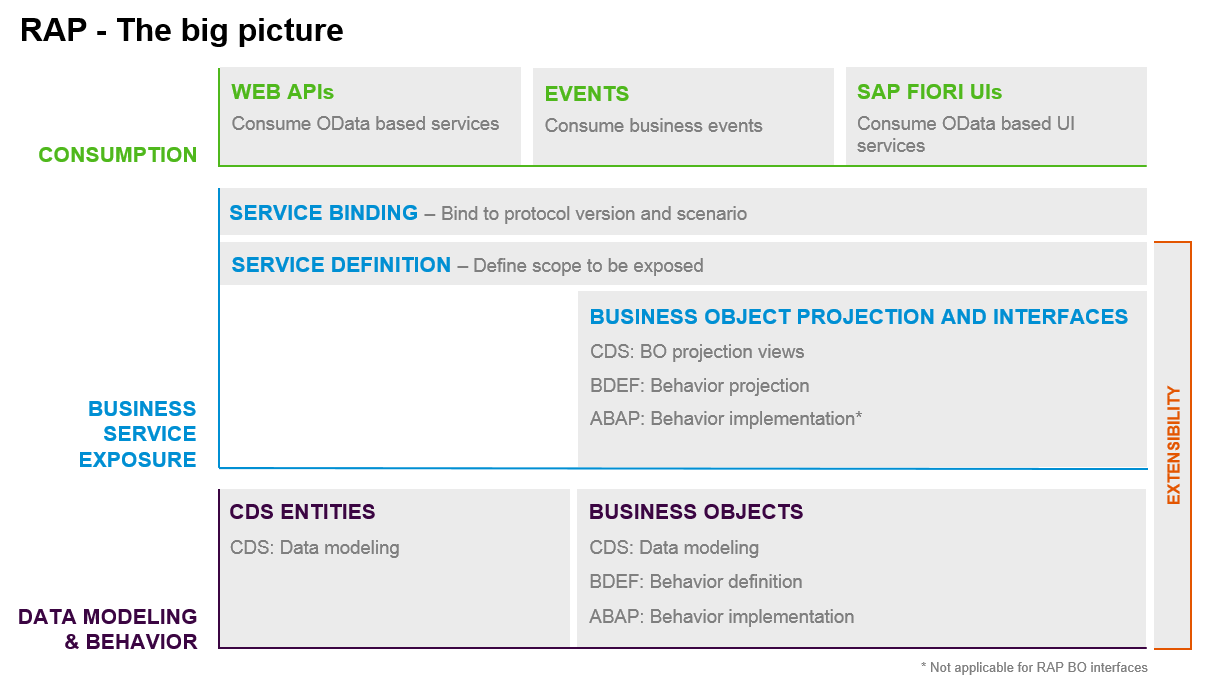
\includegraphics[height=8cm]{Bilder/RAP_Architektur.png}
    \caption[RESTful Application Programming Model Architektur]{RESTful Application Programming Model Architektur}
    \label{fig:iso_norm}
\end{figure}

Auf der untersten Ebene werden die benötigen Daten und das beabsichtigte Verhalten modelliert. Dies kann entweder durch CDS-Views oder durch Business Objects geschehen. Core Data Services sind ein Framework um das Datenmodell, basierend auf der HANA-Datenbank, zu definieren und zu organisieren. Es können selektiv die benötigten Daten aus den Datenbanktabellen ausgewählt werden. Genauer werden alle benötigten Spalten aus einer oder mehreren Tabellen ausgewählt und diese bei Bedarf  mit Annotationen versehen, um speziellere Anforderungen zu erfüllen. Es kann bei Bedarf auch noch nach Datensätzen, die gewisse Bedingungen erfüllen gefiltert werden. Somit strukturiert und gruppiert ein CDS-View die benötigten Daten. Die SQL-Abfrage, um diese Daten von der Datenbank abzurufen ist in dem CDS-View integriert. Der Zweck eines CDS-Views ist jedoch lediglich das Lesen und Strukturieren der Daten; es können hiermit keine Daten verändert werden.

Eine andere Möglichkeit ein Datenmodell zu erzeugen sind Business Objects. Diese bieten zudem die Implementierung von Behaviors (Verhalten) und einer Laufzeit. Ein BO ist aus struktureller Sicht ein hierarchisch aufgebauter Baum aus mehreren Knoten, die gewissen Daten entsprechen und durch Eltern-Kind-Beziehungen (sogenannte Kompositionen) miteinander verknüpft sind. Diese Knoten werden durch CDS Entitäten dargestellt. Der hierarchisch oberste Wurzelknoten stellt dabei die Repräsentation des BO an sich dar. Um das Verhalten eines BO zu spezifizieren, muss eine ''Business Object Behavior definition'' (''Behavior definition'' abgekürzt) angelegt werden. Dieses ABAP Objekt beschreibt das gewünschte Verhalten des BO in RAP. Die Behavior definition bezieht sich immer auf die Wurzel-CDS-Entität eines BO. Diese Behavior definition wird als ABAP Klasse implementiert. Ein Verhalten beschreibt welche Operationen und Feldeigenschaften für ein BO verfügbar sein sollen. Es besteht au{\ss}erdem noch aus der ''Behavior characteristic'', die zusätzliche Eigenschaften, wie \zB Autorisierungen für Operationen festlegt. Operationen sind \zB create() für das Erstellen, update() für das Aktualisieren und delete() für das Löschen eines Datensatzes. Diese modify-Operationen verändern im Gegensatz zu den read-Operationen auch die tatsächlichen Daten auf der Datenbank. Die Laufzeit eines BO besteht aus 2 Teilen: In der Interaktionsphase werden durch das Ausführen von Operationen Daten gelesen und/ oder verändert. Diese Veränderungen werden zunächst in einem ''transactional buffer'' (Pufferspeicher) gespeichert und nachdem alle Änderungen durchgeführt wurden in der sog. ''save sequence'' auf der Datenbank persistiert.

Die zweite Ebene sorgt für das projizieren und von BOs und die Erstellung sowie Veröffentlichung von Business Services. Ein Business Service ist in RAP ein RESTful Service, der Repräsentationen von Ressourcen veröffentlicht, die dann von Konsumenten abgerufen werden können. Die Bestandteile eines Business Services werden später noch genauer erläutert. Die Projektion eines BO ist notwendig, um es flexibel konsumieren zu können, da dieses an sich komplett unabhängig vom OData-Service ist. Das BO an sich stellt die maximal möglichen Funktionen und Daten bereit, die service-unabhängig implementiert und ggf. durch die Projektion auf die für den Service relevanten Aktionen und Daten eingeschränkt werden. Zudem können genauere Anpassungen \zB im Bezug auf die Darstellung auf einer Benutzeroberfläche über UI-Annotationen erfolgen, die aber nicht Teil des Datenmodells sein sollen. Eine zusätzliche Projektions-Schicht hat mehrere Vorteile: Zum einen kann das zugrundeliegende BO angepasst und erweitert werden, ohne dass der darauf aufbauende Service davon betroffen ist. Zum anderen können verschiedene Projektions-Views für verschiedene Anforderungen erstellt werden, die alle dasselbe BO wiederverwenden. Zudem können die Daten und Funktionen eines Services für eine Fiori App oder Web API veröffentlicht werden. Des Weiteren können Services auch rollenbaisert veröffentlicht werden, sodass unterschiedliche Daten und Funktionen für unterschiedliche Anwender bereitgestellt werden können. Um eine solche Projektionsschicht zu erstellen, muss zusätzlich eine CDS Projection View erstellt werden, um die speziellen Daten einer Projektion darzustellen. Dieser basiert auf der CDS View des BO und erzeugt selbst keine neue SQL-View, sondern nur eine Repräsentation der dargestellten Entitäten. Um eine CDS-Entität eines BO zu projizieren müssen die Wurzel-Entität sowie alle Eltern-Entitäten ebenfalls projiziert sein. Zudem wird auch eine Projection Behavior Definition benötigt, die alle Verhalten, die für einen speziellen Service veröffentlicht werden sollen projiziert.

Nachdem Teile des BO projiziert wurden und die zugehörigen Artefakte erstellt wurden, muss in der zweiten Ebene ein Service definiert werden. In einer ''business service definition'' (abgekürzt ''Service Definition'') wird festgelegt, welche CDS Entitäten eines Datenmodells, also welche Daten, in einen bestimmten Service veröffentlicht werden sollen. Die Service Definition stellt eine protokoll-unabhängige und Konsumenten-spezifische Sichtweise auf das Datenmodell dar. Es können auch mehrere CDS-Entitäten oder eine komplette BO Struktur in einem Service veröffentlicht werden. Dafür muss in der Service Definition die hierarchisch höchste Entität des BO, die veröffentlicht werden soll, markiert werden. Diese dient dann als Einstiegspunkt für den Service.

Als letzter Schritt in der zweiten Ebene muss noch das Kommunikationsprotokoll des Service im Service Binding definiert werden. Ein häufiges Beispiel wäre hierbei OData, für das Bereitstellen von Daten in einer Fiori App. Ein Service Binding bezieht sich immer direkt auf eine oder mehrere Service Definitions. Es können auch mehrere Service Bindings basierend auf einer Service Definition erstellt werden. Das ist \zB hilfreich, wenn derselbe Service mit unterschiedlichen Kommunikationsprotokollen veröffentlicht werden soll, da durch die Trennung von Service Definition und Binding das Protokoll von der Geschäftslogik getrennt wird. Somit kann der Entwicklungsaufwand für einen Service erheblich reduziert werden. Ein Service kann für die Protokolle OData Version 2 und 4 veröffentlicht werden, wenn das Ziel ist, die Daten in einer Fiori App darzustellen. OData ermöglicht au{\ss}erdem das Erstellen von HTTP-basierten Services, deren Ressourcen über URIs identifizierbar sind und über HTTP-Nachrichten abgerufen und modifiziert werden können. Dies korrespondiert wiederum mit den Designkonventionen nach REST aus dem vorhergehenden Kapitel. Zudem stehen noch die Protokolle Information Access für Analysezwecke und SQL zur Verfügung. Ein Service kann grundlegend auf zwei Arten veröffentlicht werden: Entweder als UI Service mit den Protokollen OData oder Information Access, indem man dem durch UI-Annotationen eine Fiori Elements oder andere Benutzeroberfläche hinzufügt. Für alle anderen Anwendungsfälle wird der Service als Web API veröffentlicht, die von Clients über das Web mit OData konsumiert werden kann. Wenn ein Service veröffentlicht ist, kann er jedoch im Standard nur innerhalb des Entwicklungssystems abgerufen werden. Ein Service kann zudem in mehreren Versionen existieren. Dies geschieht durch das Hinzufügen oder Entfernen von zusätzlichen Service Definitions zu einem Service Binding. Damit kann ein Service geändert oder erweitert werden.

Die dritte und oberste Ebene der RAP Architektur ist für das Konsumieren der Daten eines BO oder CDS Views verantwortlich. Es gibt zwei Möglichkeiten, diese Daten durch einen Service zu konsumieren. Die erste Möglichkeit ist durch eine Web API. Die Metadaten eines so veröffentlichten Services enthalten keine Informationen über eine Benutzeroberfläche für die Darstellung der Informationen. Der Zugriff auf die bereitgestellten Daten erfolgt über eine öffentliche Schnittstelle des OData Services. Eine weitere Möglichkeit einen Service zu konsumieren ist innerhalb einer Fiori Elements Anwendung als UI Service. Hier werden die Konfigurationen für die Benutzeroberfläche und das Front-End der Anwendung, die im Back-End als Annotationen in den CDS Entitäten festgelegt wurden, über die Metadaten mitgegeben. Somit kann das Fiori Elements Framework aus diesen Metadaten direkt eine fertige UI generieren. Als letzte Möglichkeit ein BO zu konsumieren sind noch Business Events zu nennen. Diese werden hier nur kurz genannt und in einem späteren Kapitel detaillierter beschreiben.

\section{SAP Fiori Elements}

Fiori Elements ist ein Framework zum entwickeln benutzerfreundlicher und ansprechender Anwendungen. Apps werden auf Basis von OData-Services und UI-Annotationen in den CDS Entitäten durch ein umfassendes Framework fast automatisch generiert. Somit ist im Gegensatz zur älteren SAP UI5 Freestyle Technologie kein JavaScript Coding mehr nötig um das Front-End zu programmieren. Elements benutzt vordefinierte Layouts und Controller für Aktionen der App.

Fiori Elements bietet drei zentrale Vorteile: Es soll dabei helfen, dass sich Entwickler auf die spezifische Geschäftsprozess-Logik und die Back-End Entwicklung fokussieren und somit weniger Zeit für die Programmierung der Benutzeroberfläche benötigen, was insgesamt zu einer verkürzten Entwicklungszeit von Apps und somit auch für niedrigere Entwicklungskosten sorgt. Zudem wird die Kontinuität des UI über alle Fiori Apps hinweg und die Übereinstimmung der Apps mit den SAP Designkonventionen sichergestellt. Die Benutzer der Apps haben so eine einheitliche Benutzungserfahrung (Layout, Navigation, Suche, ...) über alle Apps hinweg. Zudem stellt das zentrale Framework auch sicher, dass der Programmcode für die Benutzeroberflächen der Apps immer sofort funktioniert und bietet au{\ss}erdem weitere Funktionen wie Übersetzungen und Unterstützung für mobile Entgeräte. Diese Vorteile tragen wiederum zu einer reduzierten Entwicklungszeit und somit einem Kostenersparnis bei.

Verglichen mit SAP UI5 Freestyle (Freestyle abgekürzt), der anderen Technologie, um Fiori Apps zu entwicklen, lassen sich folgende Unterschiede feststellen: Die generelle Herangehensweise bei Fiori Elements zielt eher auf das effiziente und schnelle Entwickeln und Veröffentlichen einer App ab. Im Gegensatz dazu, liegt der Fokus bei Freestyle eher auf der Flexibilität, spezielle Anforderungen, die ggf. auch nicht mit dem Elements Standard übereinstimmen abbilden zu können. Das wirkt sich auch auf die Möglichkeiten im UI-Design aus: In Fiori Elements ist der Entwickler an die vordefinierten SAP Vorlagen gebunden, während es bei den Freestyle Designs auch möglich ist, mit einer leeren Vorlage zu beginnen. Das hat aber auch zur Folge, dass bei Freestyle wesentlich mehr Webentwicklungs Kenntnisse nötig sind, da die Oberfläche mithilfe von JavaScript Coding selbst programmiert werden muss. In Fiori Elements hingegen wird die gesamte Oberfläche vom Elements Framework generiert und muss nur durch UI-Annotationen in den CDS-Entitäten an die Wünsche des Kunden angepasst werden. Was die Wartbarkeit und entwicklungstechnischen Freiheiten der beiden Technologien angeht, sind auch bei Freestyle grö{\ss}ere Spielräume vorhanden: Dadurch, dass die Oberfläche selbst programmiert wird, ist es möglich eine Logik in das Front-End einzubauen. Diese Tatsache ist für die Problemstellung der Arbeit sehr relevant, da sequentielle Prozesse, die asynchrone Kommunikation benötigen, sich durch eben diese Logik leicht abbilden lassen. Da in Fiori Elements die das UI generiert wird und die Logik von SAP kommt, fehlt diese Gestaltungsmöglichkeit, was die Umsetzung der angesprochenen Geschäftsprozesse erschwert. Dennoch muss man sagen, dass in allen anderen Fällen Fiori Elements erhebliche Vorteile bietet, da bei der Entwicklung einer App sehr viel Zeit und somit auch Geld gespart werden kann, was somit auch die TCO reduziert. 

Beide Fiori Technologien, Elements und Freestyle verwenden das Model-View-Controller Konzept.

\begin{figure}[H]
    \centering
    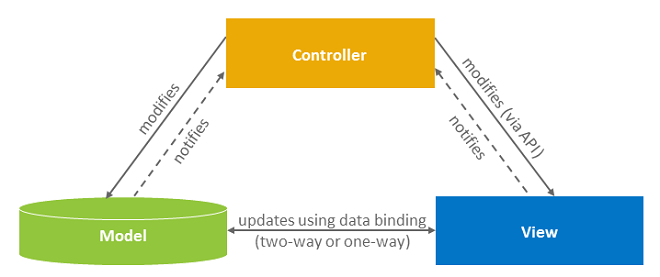
\includegraphics[height=6cm]{Bilder/Fiori_Model-View-Controller-Konzept.png}
    \caption[Model-View-Controller Konzept]{Model-View-Controller Konzept}
    \label{fig:iso_norm}
\end{figure}

Das Konzept unterteilt eine Anwendung in ein Modell, einen View und einen Controller. Das Model verwaltet die Daten der Anwendung und stellt Methoden bereit, um die Daten aus der Datenbank abzurufen und bei Bedarf zu bearbeiten. Fiori unterstützt Client- und serverseitige Modelle. Das hei{\ss}t, dass das Modell entweder komplett vom Client heruntergeladen wird und dort dann lokal existiert, oder bei serverseitigen Modellen nur die jeweils angefragten Daten vom Client beim Server angefordert werden. Wenn das Modell auf der Client Seite existieren soll, kann entweder ein JSON-, XML- oder Ressourcen-Modell verwendet werden. Serverseitig kann ein OData-Service in den Versionen zwei und vier verwendet werden. Es ist auch möglich für verschiedene Bereiche einer Anwendung jeweils verschiedene Modelle zu definieren und diesen auch modellspezifisch über den Controller verschiedene Interaktionsmöglichkeiten mit dem View zu geben. Der View definiert und rendert die Benutzeroberfläche und legt somit das Aussehen der App für den Anwender fest und visualisiert die Daten des Models. Standardmä{\ss}ig werden XML- und JSON-Views unterstützt. Zudem kann man einen View als eigene Klasse selbst programmieren. Der Controller ist für die Interaktionen des Benutzers mit der App zuständig und enthält Methoden, die die Interaktion zwischen Model und View regeln. Er enthält den Programmcode für die Geschäftsprozesslogik hinter der Anwendung. Zudem kann der Controller in Methoden oder zu bestimmten Zeitpunkten, wie \zB bei Start oder Beenden der Anwendung Events auslösen. Diese Events können dann von anderen Controllern empfangen und verarbeitet werden. Somit können eventgesteuert bestimmte Aktionen in der Anwendung ausgelöst werden. Das Ziel des Konzepts ist es, die Daten der App logisch von den Interaktionen des Benutzers zu trennen. Eine Anwendung in die genannten drei Teile aufzuteilen hat folgende Vorteile: Der Programmcode der Anwendung ist leichter lesbar, wartbar und erweiterbar, da er in logisch zusammenhängende Teile aufgeteilt ist. Somit ist es möglich die Darstellung der Daten in der View zu verändern, ohne die darunterliegende Logik oder das Datenmodell zu ändern und mit mehreren Views mehrere Darstellungsweisen, je nach Anwendungsfall zu erstellen.

Apps sind in Fiori Elements immer auf vordefinierten Layouts aufgebaut. Diese können am Anfang der Entwicklung einer App ausgewählt werden und geben das generelle Aussehen und Funktionen vor.

\begin{figure}[H]
    \centering
    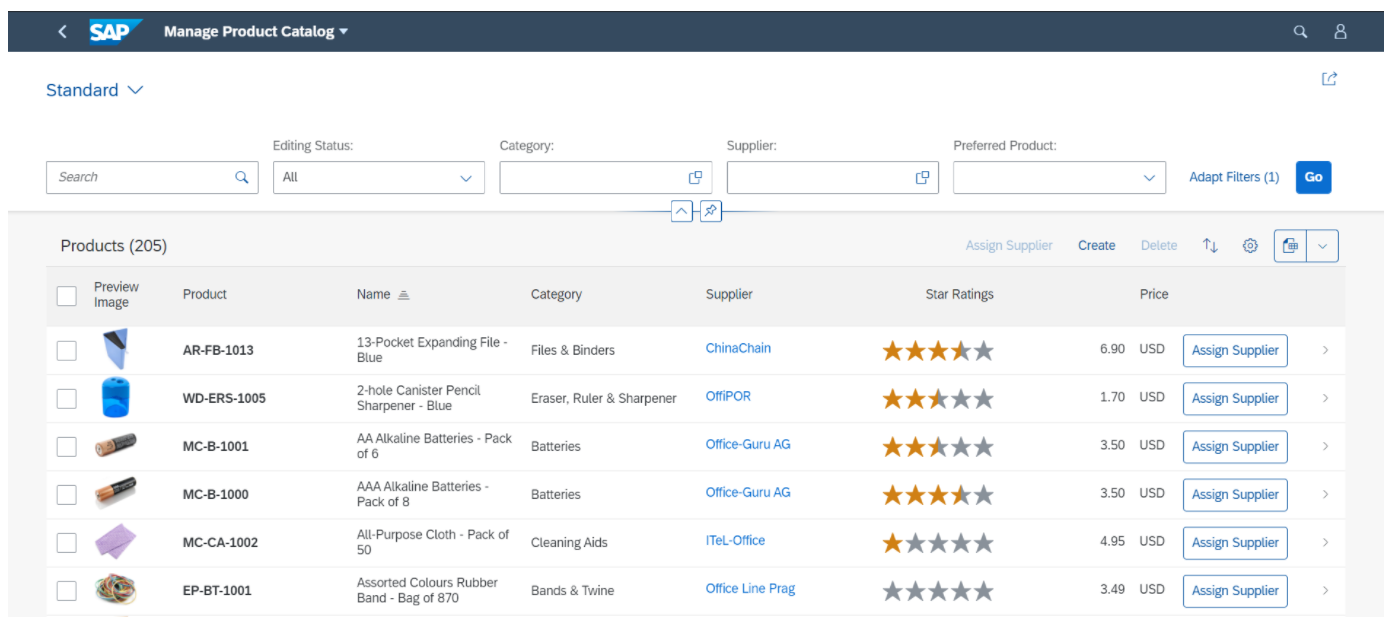
\includegraphics[height=6cm]{Bilder/Fiori_Elements_List_Floorplan.png}
    \caption[Fiori Elements List Report Floorplan]{Fiori Elements List Report Floorplan}
    \label{fig:iso_norm}
\end{figure}

Auf dem Bild ist beispielhaft das Layout List Report zu sehen. Dieser kann verwendet werden, wenn der Zweck der Anwendung das Arbeiten mit einer Liste von Dingen \zB Produkten ist. Diese werden dann in einer sortierten Tabelle dargestellt, in der der Benutzer nach Einträgen sortieren, filtern und suchen kann. Hier müssen nur die Produktdaten über einen OData Service bereitgestellt werden und die Darstellung der Daten über UI-Annotationen nach Bedarf angepasst werden. Die restliche Benutzeroberfläche mit Navigation, Suchleisten und Aktionen wird vollständig durch das Framework generiert. Der List Report wird häufig als Einstiegspunkt in einer App verwendet um nach bestimmten Objekten zu suchen und mit diesen dann in einer Object Page näher zu interagieren.

\begin{figure}[H]
    \centering
    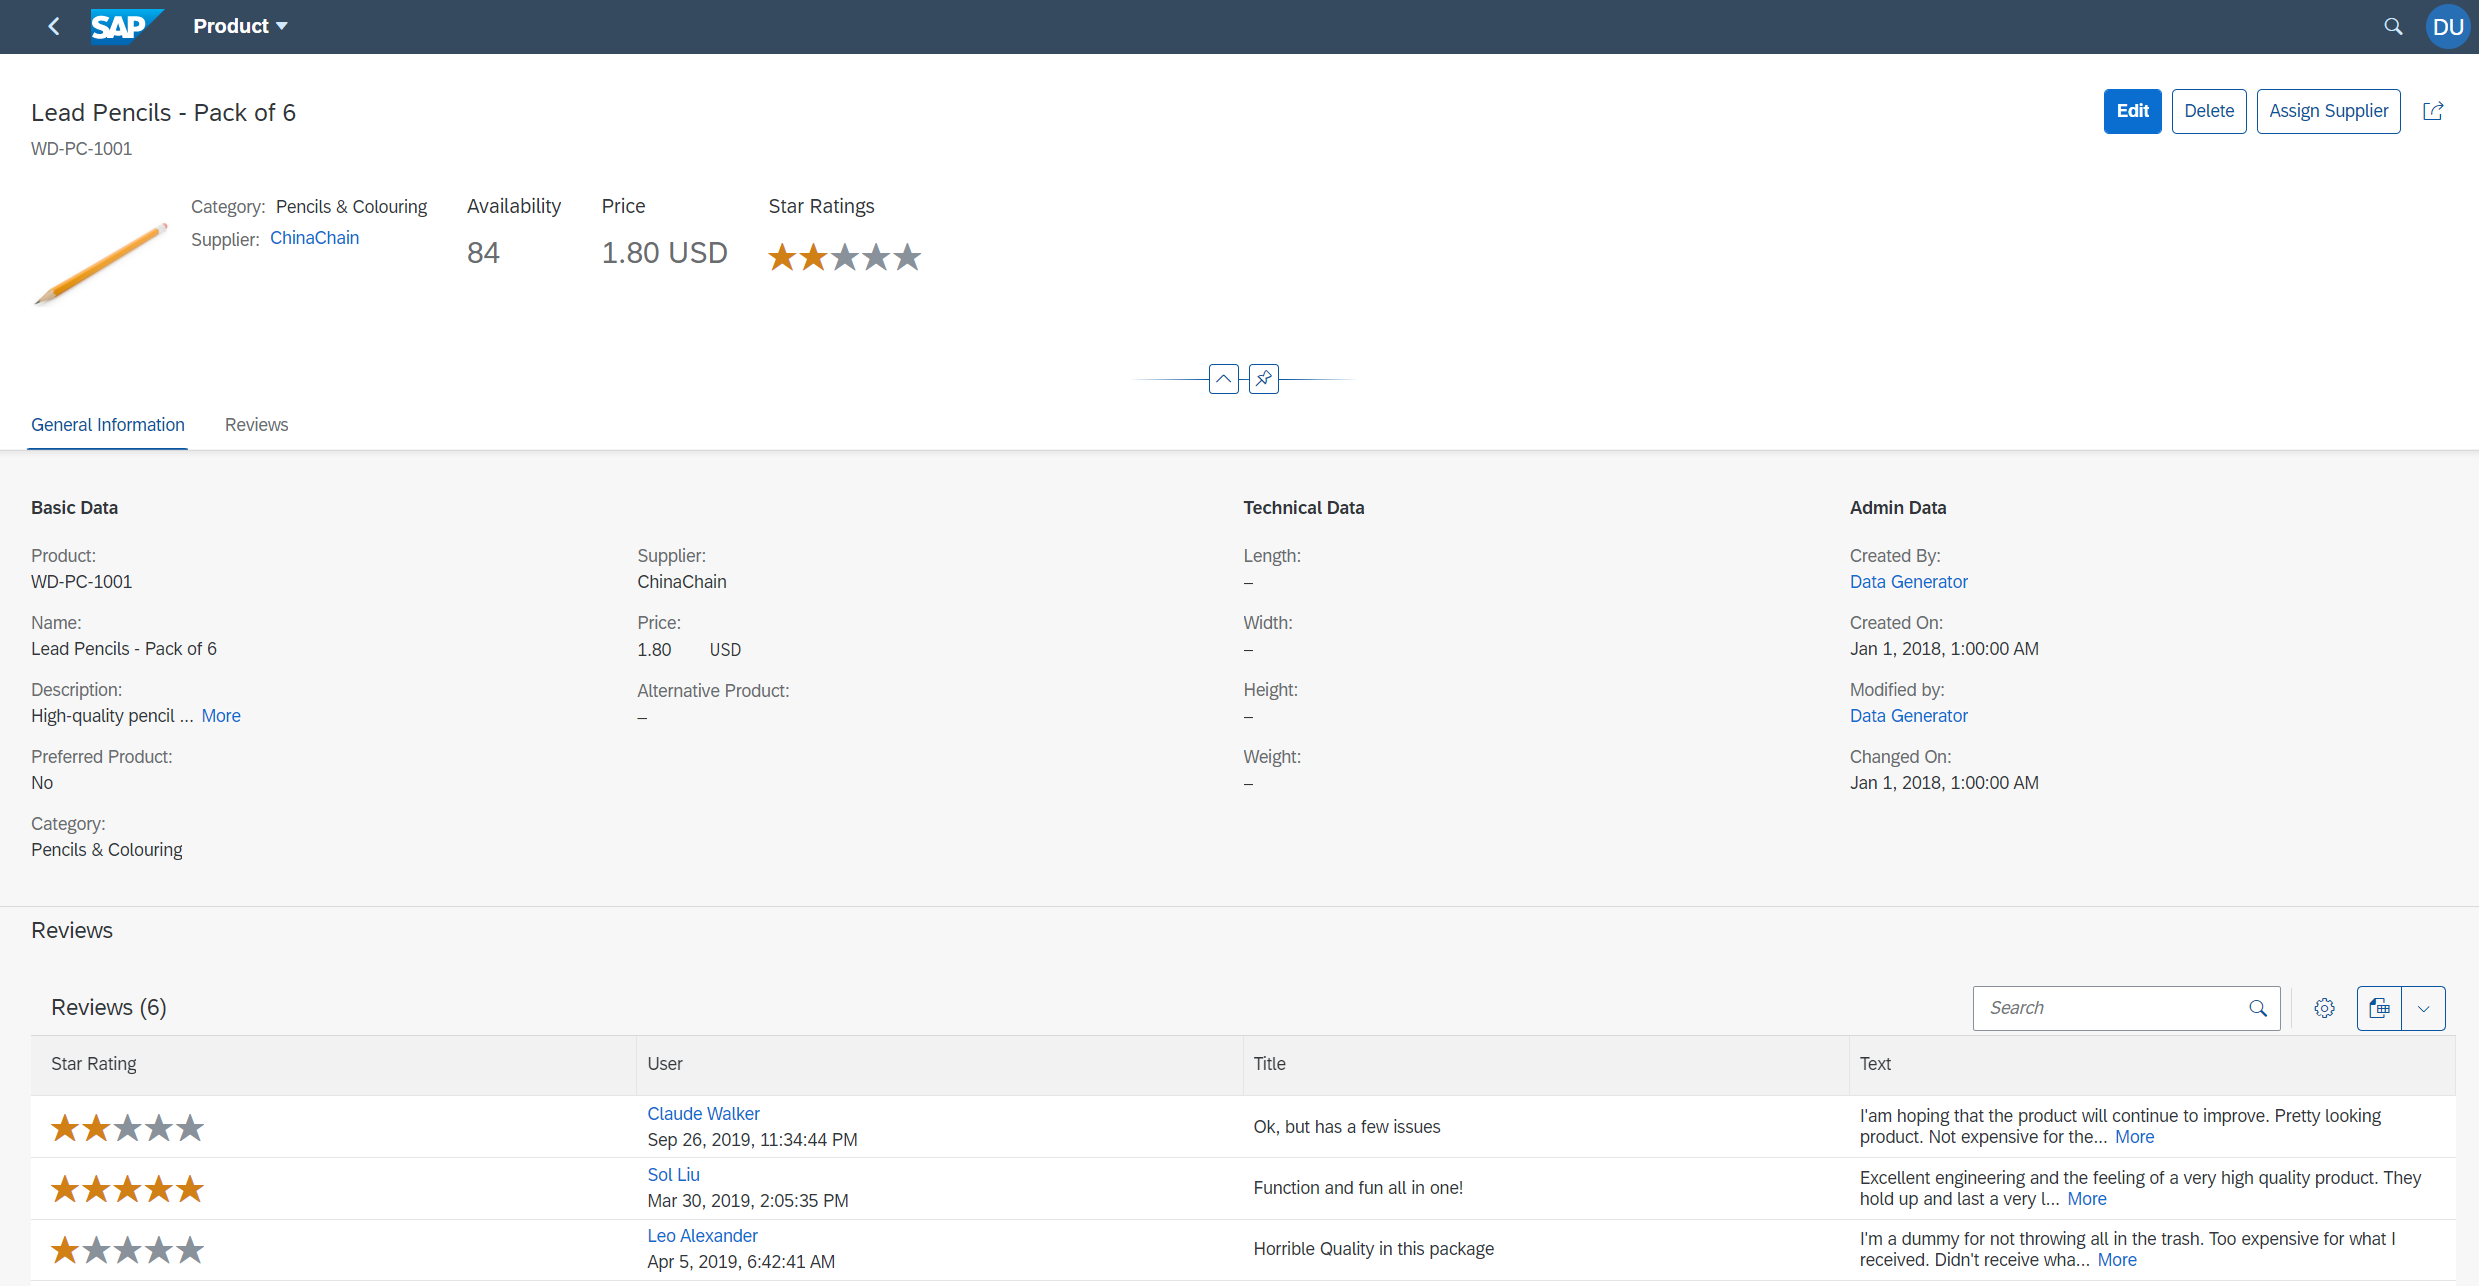
\includegraphics[height=6cm]{Bilder/Fiori_Elements_Object_Floorplan.png}
    \caption[Fiori Elements Object Page Floorplan]{Fiori Elements Object Page Floorplan}
    \label{fig:iso_norm}
\end{figure}

Das List Report Layout wird häufig mit der dem Object Page Floorplan in einer App kombiniert, wenn es darum geht, mit den einzelnen Objekten in der Liste zu arbeiten. Die Objekt-Ansicht wird durch einen Klick auf das gewünschte Objekt in der Listen-Ansicht aufgerufen. Hier können dann weitere Informationen zu \zB einem Produkt angezeigt und bei Bedarf auch bearbeitet werden. Des Weiteren gibt es noch Floorplans für eine Worklist, eine Liste mit Unterstützung für diverse Analyseverfahren, wie \zB Drill-Down und ein Dashboard.
\chapter{Praktischer Teil}

Im Folgenden werden die verschiedene praktische Lösungsansätze vorgestellt und anhand verschiedener Kriterien gegeneinander abgewogen, sodass am Ende eine Handlungsmatrix erstellt werden kann.

\section{Lösungsansätze}

Zunächst sollen drei verschiedene Technologien vorgestellt werden, mit denen sich asynchrone Prozesse mit sequentieller Kommunikation, trotz den Einschränkungen durch RAP und Fiori Elements, umsetzen lassen.

\subsection{Business Workflows}

Der erste mögliche Ansatz sind Business Workflows (BW abgekürzt). BWs können benutzt werden um jeglichen Geschäftsprozess im SAP-System abzubilden. Sie decken das Spektrum von einfachen Genehmigungsprozessen bis hin zu komplexen Abläufen ab. Sie eignen sich vor allem für repetitive Prozesse mit mehreren Bearbeitern. BWs können zudem zur Fehelerbehandlung in anderen Prozessen oder eventgesteuert eingesetzt werden. Mit Workflows können durch die Benutzung der bereits bestehenden Funktionen und Transaktionen des SAP-Systems neue Geschäftsprozesse abgebildet werden. Die Funktionen und Transaktionen an sich werden dabei durch den Workflows nicht verändert. In Kombination mit Organisationsmanagement können die einzelnen Schritte des BW durch bestimmte Akteure ausgeführt werden. Das kann auch auf bestimmte Stellen abstrahiert werden, um von personellen Veränderungen innerhalb des Unternehmens unabhängig zu sein. Workflows können auch untereinander durch das Versenden und Konsumieren von Nachrichten kommunizieren. Diese Kommunikation ist auch zwischen verschiedenen SAP-Systemen über das Internet mit XML-Dokumenten möglich. \footcite[Vgl.][]{sap_business-workflows_2022-1}

Zunächst wird die Definition der Aufbau eines Business Workflows beschrieben. Diese lässt sich in vier Bereiche unterteilen.

\begin{figure}[H]
    \centering
    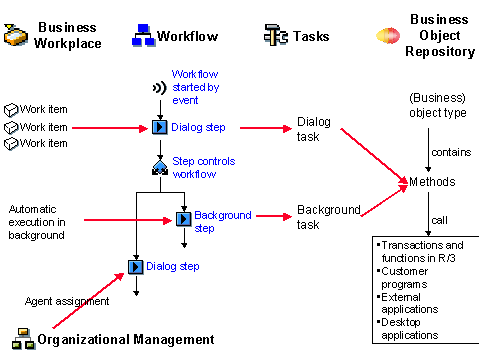
\includegraphics[height=8cm]{Bilder/Business-Workflows_Schema.png}
    \caption[Aufbau eines Business Workflows]{Aufbau eines Business Workflows, Abgerufen von \cite{sap_business-workflows_2022-1} am 17.07.2023.}
    \label{fig:iso_norm}
\end{figure}

Der Business Workplace ist der Ort in einem SAP-System, in dem der Endanwender ''work items'' (übersetzt aus dem Englischen: ''Arbeitspakete'' oder ''Aufgaben'') abhängig vom Zeitpunkt im Geschäftsprozess und den Berechtigungen des Users ausführen kann. Ein work item stellt zur Laufzeit des BW einen Schritt des Prozesses dar, der ausgeführt wird. Es werden hier jedoch nicht alle work items angezeigt. So werden \zB solche, die einem Prozess-Schritt, der im Hintergrund ausgeführt werden soll, zugeordnet sind, hier nicht angezeigt.

Ein Workflow muss vor Ausführung in der ''workflow definition'' angelegt werden. Diese Definition legt die Reihenfolge der auszuführenden Schritte des Prozesses fest und enthält zudem Kontrollschritte. Zusätzlich können noch Bearbeiter und Fristen für bestimmte Schritte festgelegt werden, die dann zur Laufzeit des Workflows vom ''Work item manager'' verwaltet werden. Es gibt viele Arten von Schritten, die gängigen Konzepten in der Programmierung ähneln, wie \zB normale Aktivitäten, Fallunterscheidungen, Schleifen. Zudem gibt es Schritte zum Versenden von Nachrichten, Auslösen von Events, Benutzerentscheidungen, usw. Diese Schritte können entweder im Dialog mit einem Benutzer ausgeführt werden, wenn \zB die Eingabe bestimmter Werte erforderlich ist, oder automatisch vom System im Hintergrund ausgeführt werden. Ein Workflow kann nicht nur manuell von einem Benutzer gestartet werden, sondern auch systemseitig von einem bestimmten Event ausgelöst werden. Hierfür muss in der Definition des Workflows das gewünschte Event als Auslöser angegeben werden. Wenn dann das Event auftritt, wird der Workflow automatisch gestartet. Im betrieblichen Kontext könnte hier \zB ein Mitarbeiter einen Urlaubsantrag stellen, der dann den als Workflow abgebildeten Genehmigungsprozess auslöst. Das wäre ein Beispiel für einen asynchronen Prozess mit sequentieller Kommunikation.

Die einzelnen Schritte, die innerhalb des Workflows ausgeführt werden, hei{\ss}en Tasks und stellen grundlegende betriebliche Tätigkeiten dar. Die Dialog- und Hintergrund-Schritte in der Workflow Definition korrespondieren hier mit Dialog- oder Hintergrund-Tasks. Im Workflow bezieht sich ein Task immer auf eine Methode eines Objekttyps. Diese Methoden können automatisch ausführbar sein oder müssen aktiv von einem Benutzer gestartet werden. Eine Methode kann einerseits Transaktionen oder Funktionen innerhalb des ERP-Systems aufrufen. Spezielle Anforderungen können durch kundeneigene Logik, oder Schnittstellen zu anderen Systemen umgesetzt werden.

Methoden, die innerhalb eines Workflows aufgerufen werden, sind immer Teil von Objekten. Diese Objekte können auch BOs sein. Im Allgemeinen ist ein Objekt ein konkreter Datensatz eines Objekttyps. Die Daten des Objekts werden durch seine Attribute definiert und die Aktionen, wie das Erstellen, Aktualisieren oder Löschen von Daten wird durch die Methoden des Objekts beschrieben. Einen weiteren wichtigen Teil von Objekten stellen Events dar. Diese werden ausgelöst, wenn bei einem Objekt seinen Status verändert. Das kann \zB durch das Erstellen, Verändern oder Löschen von Daten passieren. Diese Events können dann unter anderem Workflows starten. Das ''Business Object Repository'' bietet eine Übersicht über alle in einem SAP-System verfügbaren Objekttypen. Man kann die bereits vorhandenen Objekttypen bei Bedarf anpassen oder neue erstellen.

\subsection{Business Events}

Eine Option wären die Verwendung von Business Events. Hier auch ggf. auf Probleme mit Event-Mesh (Cloud- bzw. BTP-Komponente) für onPremise-Systeme eingehen -> lokale Verarbeitung der Business Events?

\subsection{Background Processing Framework}

Andere Option wäre das Background Processing Framework über Background remote function calls.

\section{Entscheidungsmatrix}

Hier soll eine Entscheidungsmatrix entwickelt werden, welchen Lösungsansatz man in Abhängigkeit von mehreren Faktoren am besten verwenden soll (ersetzt auch weng mit die Zusammenfassung)

Vergleichskriterien:

- BTP Event Mesh Cloud nötig in Systemlandschaft, andere Lösungen laufen nur lokal -> mehr Kosten,  Komplexität in Systemlandschaft, Datenschutz
- Kosten
- Performance (wshl verlieren BusinessEvents, Kommunikation über Systemgrenzen hinaus)
- Experteninterview: BusinessEvents (Martin Müller (+bgpf), Marcel Herrmanns, Daniel Wachs) 
\chapter{Schlussbetrachtungen}

%Im folgenden sollen die wichtigsten Ergebnisse noch einmal zusammengefasst werden. Zudem soll eine Handlungsempfehlung gegeben und die Arbeit einmal kritisch reflektiert werden. Abgeschlossen wird mit einem Ausblick auf weitere Entwicklungen.

\section{Zusammenfassung}

Die wissenschaftliche Arbeit beschäftigt sich mit der Umsetzung sequentieller Prozesse im RESTful-Umfeld und vergleicht verschiedene praktische Lösungsansätze in SAP-Systemen. 

Der theoretische Teil der Arbeit führt in die Grundlagen von RESTful-APIs mit Designprinzipien wie einer Client-Server-Architektur, Zustandslosigkeit, Caching, einer einheitlichen Schnittstelle und Schichtenarchitektur ein, erläutert die Architektur des ABAP RESTful Application Programming Model und stellt SAP Fiori Elements als Framework für das einfache Entwickeln einheitlicher, ansprechender Apps vor. \newline
Der praktische Teil untersucht drei Ansätze für die Abbildung asynchroner Prozesse mit sequentieller Kommunikation: Business Workflows, Business Events und das Background Processing Framework (bgPF). Workflows ermöglichen die Abbildung verschiedener Geschäftsprozesse im SAP-System und eignen sich für repetitive Prozesse. Business Events ermöglichen asynchrone Kommunikation zwischen Business Objects, während das bgPF die Auslagerung von Logik in separate Prozesse erlaubt.

Die Vergleichsanalyse zeigt, dass Workflows potenziell komplex sind, während Business Events je nach Ansatz variieren und das bgPF eher einfach einzusetzen ist. In Bezug auf die Systemlandschaft benötigen Workflows keine zusätzlichen Anforderungen, während Business Events und bgPF spezifische Broker bzw. Event Meshes erfordern. Workflows zeigen gute Performance, jedoch können Benutzerinteraktionen die Ausführung blockieren. Business Events sind effizient, aber die Grö{\ss}e der Daten kann die Performance beeinflussen, während das bgPF durch seine asynchrone Natur eine gewisse Verzögerung aufweist. Die Kosten variieren bei den Ansätzen: Workflows und das bgPF verursachen keine zusätzlichen Kosten, während Business Events Investitionen erfordern können. Hinsichtlich Flexibilität bieten Workflows und das bgPF Anpassungsmöglichkeiten durch ABAP-Coding, während Business Events ebenfalls anpassbar sind und gut in die Systemlandschaft integriert werden können. In Bezug auf Skalierbarkeit zeigen Workflows nur lineares Wachstum, Business Events sind sehr gut skalierbar, während das bgPF hier derzeit noch Defizite im Bezug auf die Skalierbarkeit hat und ausschlie{\ss}lich in Cloud-Systemen verfügbar ist. Die Wartbarkeit von Workflows und dem bgPF ist relativ einfach, während Business Events von der korrekten Implementierung abhängig sind, aber gut gewartet werden können. Abschlie{\ss}end wird die Abwärtskompatibilität betrachtet: Workflows sind sehr gut abwärtskompatibel, während Business Events und bgPF von der verwendeten Technologie und Version abhängen. Workflows bieten sich somit an, wenn Abwärtskompatibilität wichtig ist.

In der Entscheidungsmatrix zeigt sich, dass Workflows breite Stärken haben, Business Events besonders skalierbar und effizient sind, während das bgPF Framework besonders für Cloud-Systeme geeignet ist. Alle drei Ansätze sind je nach spezifischem Anwendungsszenario nutzbar.

\section{Handlungsempfehlung}

Abschlie{\ss}end soll eine Handlungsempfehlung für den konkreten Anwendungsfall in der Abteilung gegeben werden. Die nachfolgende Tabelle stellt eine gewichtete Entscheidungsmatrix der Kriterien, anhand derer die verschiedenen Ansätze verglichen wurden, dar.

% \begin{figure}[H]
%  \centering
%  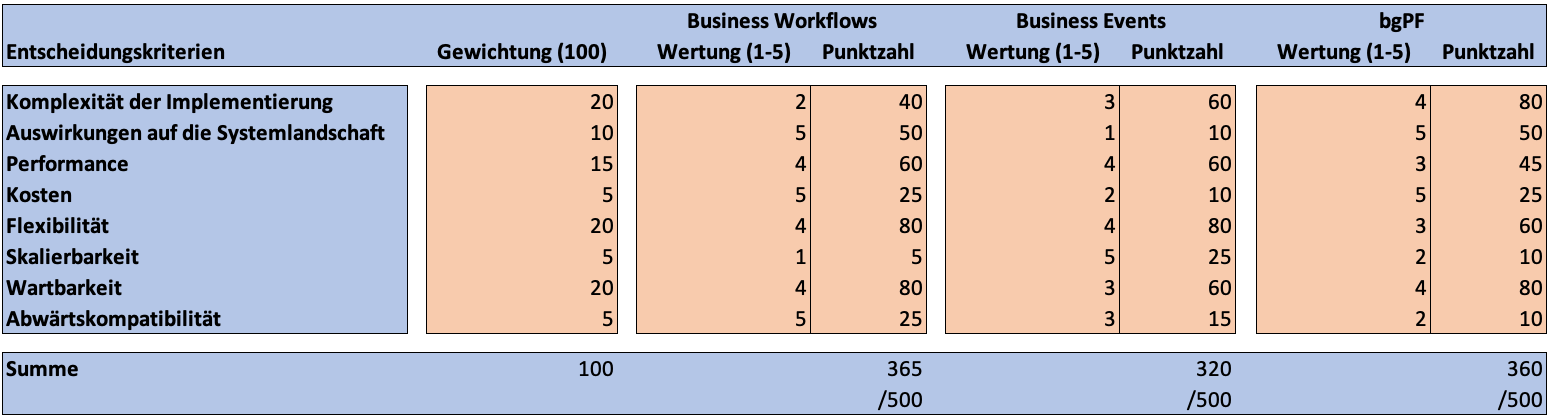
\includegraphics[height=4.06cm]{Bilder/Handlungsempfehlung_Entscheidungsmatrix.png}
%  \caption[gewichtete Entscheidungsmatrix der drei Ansätze]{gewichtete Entscheidungsmatrix der drei Ansätze, eigene Darstellung}
%  \label{fig:iso_norm}
% \end{figure}

\begin{table}[h]
    \centering
    \begin{tabular}{c}
        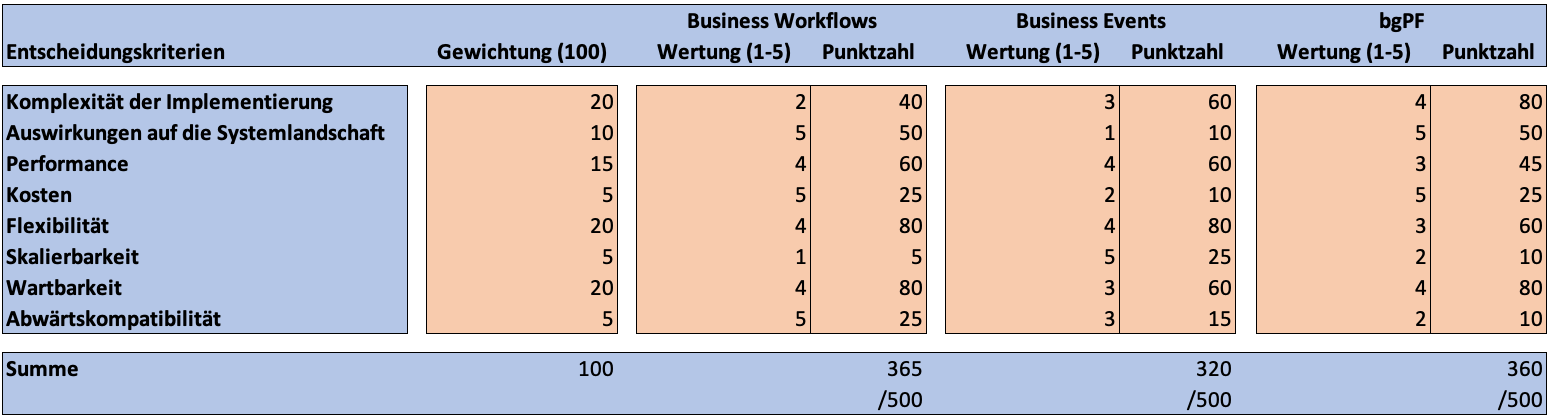
\includegraphics[height=4cm]{Bilder/Handlungsempfehlung_Entscheidungsmatrix.png}
    \end{tabular}
    \caption[Gewichtete Entscheidungsmatrix der drei Ansätze]{Gewichtete Entscheidungsmatrix der drei Ansätze. eigene Darstellung}
    \label{tab:iso_norm_Entscheidungsmatrix}
\end{table}


Die Gewichtungen der Kriterien wurden durch eine abteilungsinterne Befragung der für das Thema verantwortlichen Personen ermittelt. Die Wertungen der Technologien für die einzelnen Vergleichspunkte wurden aus dem Vergleich im vorhergehenden Kapitel bestimmt. Somit ergibt sich, dass die Technologie Business Workflows, die auch aktuell zum Lösen der Problemstellung im Betrieb zum Einsatz kommt tatsächlich, entgegen der anfänglichen Annahme die beste Variante ist, wenn auch der Unterschied zum bgPF nur sehr marginal ist (Vgl. Abb. \ref{fig:iso_norm_Diagramm}). Da die Bewertungen relativ zueinander erfolgt sind, bei den beiden Technologien nur um 1\% abweichen und generell ähnliche Stärken haben, sollten diese als gleichwertig geeignet für die Lösung der Problemstellung betrachtet werden. Business Events würden sich zwar grundlegend auch für den Anwendungsfall eigenen, bieten aber insgesamt nicht so viele Vorteile wie die anderen beiden Ansätze. Allgemein hängt die Wahl von der spezifischen Gewichtung der einzelnen Kriterien ab. 

\section{Reflexion der Arbeit und Ausblick}

Die anfängliche Fragestellung der Arbeit war, welcher der drei vorgestellten Lösungsansätze am besten im betrieblichen Anwendungsszenario eingesetzt werden sollte und welcher Ansatz sich allgemein anhand mehrerer Vergleichskriterien wofür eignet. Im letzten Kapitel des Praxisteils und im vorhergehenden Kapitel der Arbeit wurden diese Fragen nun beantwortet. Es wurde gezeigt welcher Ansatz für die Abteilung der geeignetste wäre sowie allgemein die Stärken und Schwächen der einzelnen Ansätze herausgestellt, sodass die Ergebnisse ohne Weiteres auch auf andere ähnliche Szenarien übertragen werden können. Möglichkeiten der weitergehenden Forschung bestehen vor allem darin, die vorgestellten Ansätze anhand von Prototypen oder Proof-of-Concepts in der Praxis anzuwenden und somit auch eine praktische Referenz für die Umsetzung sequentieller Prozesse im RESTful-API Umfeld mit einem transaktionalen Kontext zu bilden. Des Weiteren können auch noch weitere Ansätze zur Umsetzung solcher Prozesse betrachtet werden, die in dieser Arbeit aufgrund des Umfangs keine Berücksichtigung finden konnten.

% ---- Literaturverzeichnis
\cleardoublepage
\renewcommand*{\chapterpagestyle}{plain}
\pagestyle{plain}
% \pagenumbering{Roman}                   % Römische Seitenzahlen
% \setcounter{page}{\numexpr\value{savepage}+1}

\printbibliography[title = Literaturverzeichnis]

% ---- Anhang
\appendix
%\clearpage
%\pagenumbering{Roman}  % römische Seitenzahlen für Anhang

\newpage
\end{document}
